\documentclass[final,3p,times]{elsarticle}
\usepackage[T1]{fontenc}
\usepackage{lmodern,amsmath,amssymb,amsthm,booktabs,graphicx,microtype,tabularx,placeins,float,longtable}
\usepackage[colorlinks=true,linkcolor=black,citecolor=black,urlcolor=blue]{hyperref}
\setlength{\emergencystretch}{2em}
\renewcommand{\thesection}{S\arabic{section}}
\renewcommand{\thetable}{S\arabic{table}}
\renewcommand{\thefigure}{S\arabic{figure}}
\renewcommand{\theequation}{S\arabic{equation}}
\graphicspath{{figures/}}
\begin{document}
\begin{frontmatter}
\title{Supplementary Material: Executable Operating Contracts Linking Anytime Localization to Engineering Task Evidence}
\author[ae]{Chuansu Peng}
\author[ae]{Haoran Dong}
\author[ae]{Ruoxuan Wu}
\author[etc]{Peipei Zeng}
\address[ae]{School of Aeronautical Engineering, Civil Aviation University of China, China}
\address[etc]{Engineering Training Center, Civil Aviation University of China, China}
\end{frontmatter}
\suppressfloats[t]
\section{Prospective protocol and execution provenance}\label{supp:r8-protocol}
This section concerns the R8 prospective study. The later sections labelled retained describe earlier A19/A20, R4 and secondary R5 studies with their original populations, confidence families and timing. They are not pooled with R8. All complete original manuscripts/source archives remain in the release.

\begin{table}[!htbp]\centering\small
\caption{Disjoint R8 seed blocks. A seed is one independent geometric episode input, not one policy execution.}\label{supp:r8-seeds}
\begin{tabular}{@{}lrrl@{}}\toprule
Block & First seed & Inputs & Role\\\midrule
Excluded pilot &8,200,000&48&Characterization/software audit\\
Nominal calibration &8,300,000&4,096&Cards and catalogue selection\\
Unfitted calibration &8,400,000&4,096&Separate cards, unchanged predictor\\
Nominal confirmation &8,500,000&2,048&Independent frozen comparisons\\
Unfitted confirmation &8,600,000&2,048&Independent transfer comparisons\\
Occlusion stress &8,700,000&384&Unsupported descriptive stress\\
Degeneracy stress &8,800,000&384&Unsupported descriptive stress\\
Prior-shift stress &8,900,000&384&Unsupported descriptive stress\\
Map-shift stress &9,000,000&384&Unsupported descriptive stress\\\bottomrule
\end{tabular}
\end{table}

Nominal and unfitted populations are uniform discrete mixtures of their listed geometry, prior deviation, noise and discrepancy settings, with independent perturbation/noise draws per seed. A certificate concerns the entire mixture, not each constituent subgroup. Repeated source frames are permitted draws from the fixed route-template population; independently realized sensor/prior/motion perturbations remain the experimental unit. Geometry and template hashes define conditional simulation artifacts rather than a census of physical aircraft variability.

\subsection{F0, attachment amendment and F1}
F0 at 2026-10-11 19:07:18.664676 UTC binds 48 numerical/model/artifact components plus the protocol, characterized clock and preflight audit. No final input existed at F0. Frozen predictors are retained CART/RF exports fitted on the earlier 926/194 source-grouped train/validation split; no new input refits either predictor. A19/A20 and R4/R5 data are separate retained studies.

The source-history guard is an explicitly post-F0, pre-F1 attachment amendment. V1 (19:33:16 UTC) demonstrated numerical noninterference but allowed a freshly reconstructed procedural ledger to reset the same source's latch. Independent statistical review identified this discrepancy. V2 introduced persistent scope state; further provenance/timer edits were completed before a final V3 seal at 19:46:40.196132 UTC. Intermediate manifests, matching snapshots, review evidence and superseded status are retained. None was used to generate confirmation data or select a policy. F0, the deterministic event map and family size were unchanged. V3 independently seals the observer, its verification script, integrated confirmation driver and F1 binder.

F1 at 19:59:17.439444 UTC seals 528 real calibration cards, all 96 request plans, calibration means, runtime bindings and calibration-result/input hashes. A preconfirmation inventory at 19:59:32.211933 UTC verified exactly 8,192 raw calibration files and no confirmation/stress files; the separate F1--V3 binding followed at 19:59:32.903035 UTC. Confirmation generation began afterward. These local hashes and execution logs expose chronology but are not external preregistration. The gate-correction note recorded 26 route files present when that later correction was made, a progress snapshot rather than the preconfirmation or final inventory; the final release contains all 36. The executed gate used an incorrect singular route filename; its original source and inventory are preserved, the future glob is corrected, and the independent generation ledger establishes actual route chronology. Two missing unfitted-confirmation JSONL records were restored by rerunning the unchanged collector on their original seeds; all 15 arrays and full NPZ hashes match preserved originals exactly. Their lost original prefix CPU metadata is replaced by recovery-time CPU measurement, not claimed to be bytewise recovered. No source was omitted or added.

\subsection{Exact binomial family and sensitivity}
For each of 22 complete policies, two profiles, four services and three events, one independent source contributes one binary failure. The corrected one-sided tail is $\beta/K=0.05/528$. For $k<n$, inversion of the binomial lower-tail equation gives $U=\operatorname{Beta}^{-1}(1-\beta/K;k+1,n-k)$; for $k=n$, $U=1$. For $k=0$, $U=1-(\beta/K)^{1/n}$. The card loader recomputes the inversion and checks finite bounds, integer counts, $K$, $\beta$ and sealed body identity.

Cross-policy/service/event dependence does not reduce the source count and is allowed by the union-bound proof. Four requested tasks and three allowances query the same pre-frozen event cards and add no new event family. The union event is evaluated directly from the two binary failures. Two marginals cannot be substituted for that union guarantee. No route failure, fault-injection fixture or receipt-conditioned subset is added to these denominators.

Nested calibration prefixes 128/256/512/1024/2048/4096 and confidence 0.90/0.95/0.99 recompute diagnostic bounds for the unchanged 528-member family. They do not change F1 or optimize the final sample size. Raw and summary tables contain count, upper bound, requested allowance, signed margin and certified-policy count for every combination. Negative margin means refusal. A small positive margin is not silently promoted to robust support.

\subsection{Work-clock versus native CPU}
The pilot characterizes deterministic CPU-equivalent operation coefficients. Solver initialization, correspondence calls and checkpoint costs fit counted native prefixes; foreground voxel processing uses $n\log_2(1+n)$, forecast work counts tree traversals, and propagation/publication/checking primitives are separately timed. The fitted clock is conditioned on its fixed pilot estimate during calibration. It is a simulated service convention with mean costs and timestamp quantization, not measured embedded latency or worst-case execution time.

The hard sender budget includes source seals, ICP/features, forecasting, rule evaluation and publication witnesses. A common next-stage reservation assumes at most six correspondence queries per new iteration plus checkpoint/model/rule/publication work. Frontend and stream/receiver work are outside that stage cap but inside total work and availability. If the next stage is unaffordable, the last eligible candidate may publish; otherwise the service retains its prior. This wrapper changes even fixed-cap behavior, so all cards are newly calibrated effective policies.

Controlled policy traces execute one common native ICP prefix per input and charge its selected prefix to each counterfactual. Rule decisions, source sealing, producer witnesses, validation and motion replay execute for each service/policy. The integrated wrapper's component ledger adds measured claim bookkeeping; its additional inclusive replay ledger includes offline truth assertions and scoring and is explicitly not pure online CPU. Metadata-only R4/R5 microbenchmarks measure different operations and are not added as an end-to-end improvement.

For complete routes, the entire online loop is measured directly, including array copies, frontend, registration/features, forecasting, precommit/dispatch, producer/receiver checks, replay and scheduling. A versioned input-provider wrapper hydrates compressed raw arrays before the original online timer, avoiding lazy archive decompression inside service timing. Numerical arrays and the frozen route executor are unchanged. A paired provider audit checks complete numeric/clock/event traces. Startup and archive-hydration CPU are recorded separately in worker manifests. CPU is native process time on the documented host; total simulated route duration is not a throughput or embedded real-time measurement.

\subsection{Inference and descriptive analyses}
The 16 primary intervals use standard service and both confirmation profiles, loss and observation failure, for Full--validated Flat and KG1--FlatCART/FlatRF/Fixed2. The Full/Flat request is union at allowance 0.15. A refused source retains its prior and stays in the denominator. With 32,000 paired bootstrap replicates, the pointwise interval uses quantiles 0.025/0.975 and the family-adjusted interval uses $0.05/(2\times16)$ and its complement. Both are approximate percentile intervals, unlike exact binomial calibration. Input seeds, not repeated policies or time samples, are resampled.

Stress, subgroups, Pareto fronts, route replicates, influence deletion and tail order statistics are descriptive. The 36 route inputs have four paired realizations per geometry/condition with predeclared discrepancy/noise combinations; they are not assumed identically distributed replicates of one mixture. Raw route points and paired replicate differences remain available rather than receiving episode-based confidence claims. The diagnostic route is fixed to unfitted geometry/contention/replicate zero, not selected for a favorable curve.

\subsection{Mechanism assumptions and failure conditions}
Source replacement requires a common immutable prior, a retained solve and no interleaved independent update. Attachment assumes trusted producer records and startup card validation, matched active dependencies, pre-sensing commitment and canonical modeled delivery/replay. The history monitor covers rejected operational version attempts associated with the trusted source scope. A normal deadline expiry, empty catalogue or ordered rollback is not a history fault. Once faulted, the source cannot reset its attachment by reconstructing a plan or ledger. Its independent successor scope can still operate.

Fingerprint equality does not detect physical drift, authenticate compromised code or validate a sampling mixture from metadata alone. Undetected missing packets, future motion substituted for causal replay, physical processor delays, changed model/service semantics and external interleaved measurements require revised assumptions or calibration. Remaining authorized receipts do not define a conditionally calibrated subpopulation. The original candidate descriptors in the F0 trace remain reproducibility records; only V3 final receipts are the guarded public attachment.

\subsection{Dependency-lifetime software fixtures}
The excluded preflight changes one active dependency at a time and queries the same 528-card registry. Replacing the RF forecast revokes 168 cards, nominal geometry artifacts 264, the union-event definition 176, standard-service definition 132 and the common clock 528. These are constructed dependency tests, not new population failures or a claim of superiority over a procedural implementation with the same dependency validation. Previously serialized assessment objects remain historical snapshots; eligibility must be checked again at current issuance/use.

\section{Prospective result tables and additional figures}\label{supp:r8-results}
All tables below are derived from completed frozen R8 records. Controlled policy outcomes share independent inputs; integrated task executions and route variants are paired repetitions. Counts and units are kept separate from the later retained historical study. Complete precision, every price variant and all CPU/event fields are available in the CSV tables and raw journals.
\subsection{All primary calibration cards}
Each row has n=4,096 for each event and K=528. T/O/U mean trajectory/observation/direct union; margins use allowance 0.15. No card is removed because its margin is negative. All policies are freshly calibrated under the common budget wrapper.
\small\begin{longtable}{@{}llrrrrrrr@{}}
\caption{Nominal calibration: failure counts, exact corrected upper bounds and union margin.}\label{supp:cards-nominal}\\\toprule
Service & Policy & $k_T$ & $k_O$ & $k_U$ & $U_T$ & $U_O$ & $U_U$ & Margin\\\midrule\endfirsthead
\toprule
Service & Policy & $k_T$ & $k_O$ & $k_U$ & $U_T$ & $U_O$ & $U_U$ & Margin\\\midrule\endhead
relaxed & KG0.3 & 228 & 237 & 283 & 0.07022 & 0.07266 & 0.08503 & +0.06497\\
relaxed & KG1 & 244 & 229 & 278 & 0.07455 & 0.07049 & 0.08369 & +0.06631\\
relaxed & KG3 & 281 & 230 & 285 & 0.08450 & 0.07077 & 0.08557 & +0.06443\\
relaxed & FlatCART0.3 & 228 & 237 & 283 & 0.07022 & 0.07266 & 0.08503 & +0.06497\\
relaxed & FlatCART & 244 & 229 & 278 & 0.07455 & 0.07049 & 0.08369 & +0.06631\\
relaxed & FlatCART3 & 281 & 230 & 285 & 0.08450 & 0.07077 & 0.08557 & +0.06443\\
relaxed & FlatRF0.3 & 217 & 226 & 267 & 0.06724 & 0.06968 & 0.08074 & +0.06926\\
relaxed & FlatRF & 244 & 220 & 269 & 0.07455 & 0.06805 & 0.08128 & +0.06872\\
relaxed & FlatRF3 & 283 & 231 & 286 & 0.08503 & 0.07104 & 0.08584 & +0.06416\\
relaxed & ContractRF0.3 & 217 & 226 & 267 & 0.06724 & 0.06968 & 0.08074 & +0.06926\\
relaxed & ContractRF & 244 & 220 & 269 & 0.07455 & 0.06805 & 0.08128 & +0.06872\\
relaxed & ContractRF3 & 283 & 231 & 286 & 0.08503 & 0.07104 & 0.08584 & +0.06416\\
relaxed & Fixed2 & 333 & 284 & 338 & 0.09835 & 0.08530 & 0.09968 & +0.05032\\
relaxed & Fixed4 & 216 & 257 & 298 & 0.06697 & 0.07805 & 0.08904 & +0.06096\\
relaxed & Fixed8 & 216 & 257 & 298 & 0.06697 & 0.07805 & 0.08904 & +0.06096\\
relaxed & Fixed16 & 216 & 257 & 298 & 0.06697 & 0.07805 & 0.08904 & +0.06096\\
relaxed & Final & 216 & 257 & 298 & 0.06697 & 0.07805 & 0.08904 & +0.06096\\
relaxed & Residual & 331 & 278 & 332 & 0.09782 & 0.08369 & 0.09809 & +0.05191\\
relaxed & Random2or4 & 275 & 266 & 310 & 0.08289 & 0.08047 & 0.09224 & +0.05776\\
relaxed & OldRAVC & 279 & 227 & 283 & 0.08396 & 0.06995 & 0.08503 & +0.06497\\
relaxed & CART\_Time & 244 & 229 & 278 & 0.07455 & 0.07049 & 0.08369 & +0.06631\\
relaxed & RF\_Time & 244 & 220 & 269 & 0.07455 & 0.06805 & 0.08128 & +0.06872\\
standard & KG0.3 & 226 & 211 & 263 & 0.06968 & 0.06560 & 0.07967 & +0.07033\\
standard & KG1 & 242 & 209 & 263 & 0.07401 & 0.06506 & 0.07967 & +0.07033\\
standard & KG3 & 281 & 228 & 286 & 0.08450 & 0.07022 & 0.08584 & +0.06416\\
standard & FlatCART0.3 & 226 & 211 & 263 & 0.06968 & 0.06560 & 0.07967 & +0.07033\\
standard & FlatCART & 242 & 209 & 263 & 0.07401 & 0.06506 & 0.07967 & +0.07033\\
standard & FlatCART3 & 281 & 228 & 286 & 0.08450 & 0.07022 & 0.08584 & +0.06416\\
standard & FlatRF0.3 & 333 & 285 & 341 & 0.09835 & 0.08557 & 0.10048 & +0.04952\\
standard & FlatRF & 333 & 285 & 341 & 0.09835 & 0.08557 & 0.10048 & +0.04952\\
standard & FlatRF3 & 333 & 285 & 341 & 0.09835 & 0.08557 & 0.10048 & +0.04952\\
standard & ContractRF0.3 & 333 & 285 & 341 & 0.09835 & 0.08557 & 0.10048 & +0.04952\\
standard & ContractRF & 333 & 285 & 341 & 0.09835 & 0.08557 & 0.10048 & +0.04952\\
standard & ContractRF3 & 333 & 285 & 341 & 0.09835 & 0.08557 & 0.10048 & +0.04952\\
standard & Fixed2 & 333 & 285 & 341 & 0.09835 & 0.08557 & 0.10048 & +0.04952\\
standard & Fixed4 & 214 & 239 & 284 & 0.06642 & 0.07320 & 0.08530 & +0.06470\\
standard & Fixed8 & 214 & 239 & 284 & 0.06642 & 0.07320 & 0.08530 & +0.06470\\
standard & Fixed16 & 214 & 239 & 284 & 0.06642 & 0.07320 & 0.08530 & +0.06470\\
standard & Final & 214 & 239 & 284 & 0.06642 & 0.07320 & 0.08530 & +0.06470\\
standard & Residual & 331 & 278 & 335 & 0.09782 & 0.08369 & 0.09889 & +0.05111\\
standard & Random2or4 & 275 & 258 & 307 & 0.08289 & 0.07832 & 0.09144 & +0.05856\\
standard & OldRAVC & 279 & 226 & 285 & 0.08396 & 0.06968 & 0.08557 & +0.06443\\
standard & CART\_Time & 242 & 209 & 263 & 0.07401 & 0.06506 & 0.07967 & +0.07033\\
standard & RF\_Time & 333 & 285 & 341 & 0.09835 & 0.08557 & 0.10048 & +0.04952\\
tight & KG0.3 & 536 & 3054 & 3079 & 0.15152 & 0.77053 & 0.77641 & -0.62641\\
tight & KG1 & 536 & 3054 & 3079 & 0.15152 & 0.77053 & 0.77641 & -0.62641\\
tight & KG3 & 536 & 3054 & 3079 & 0.15152 & 0.77053 & 0.77641 & -0.62641\\
tight & FlatCART0.3 & 536 & 3054 & 3079 & 0.15152 & 0.77053 & 0.77641 & -0.62641\\
tight & FlatCART & 536 & 3054 & 3079 & 0.15152 & 0.77053 & 0.77641 & -0.62641\\
tight & FlatCART3 & 536 & 3054 & 3079 & 0.15152 & 0.77053 & 0.77641 & -0.62641\\
tight & FlatRF0.3 & 536 & 3959 & 3961 & 0.15152 & 0.97607 & 0.97648 & -0.82648\\
tight & FlatRF & 536 & 3959 & 3961 & 0.15152 & 0.97607 & 0.97648 & -0.82648\\
tight & FlatRF3 & 536 & 3959 & 3961 & 0.15152 & 0.97607 & 0.97648 & -0.82648\\
tight & ContractRF0.3 & 536 & 3959 & 3961 & 0.15152 & 0.97607 & 0.97648 & -0.82648\\
tight & ContractRF & 536 & 3959 & 3961 & 0.15152 & 0.97607 & 0.97648 & -0.82648\\
tight & ContractRF3 & 536 & 3959 & 3961 & 0.15152 & 0.97607 & 0.97648 & -0.82648\\
tight & Fixed2 & 536 & 2983 & 3008 & 0.15152 & 0.75378 & 0.75968 & -0.60968\\
tight & Fixed4 & 536 & 2983 & 3008 & 0.15152 & 0.75378 & 0.75968 & -0.60968\\
tight & Fixed8 & 536 & 2983 & 3008 & 0.15152 & 0.75378 & 0.75968 & -0.60968\\
tight & Fixed16 & 536 & 2983 & 3008 & 0.15152 & 0.75378 & 0.75968 & -0.60968\\
tight & Final & 536 & 2983 & 3008 & 0.15152 & 0.75378 & 0.75968 & -0.60968\\
tight & Residual & 536 & 2983 & 3008 & 0.15152 & 0.75378 & 0.75968 & -0.60968\\
tight & Random2or4 & 536 & 2983 & 3008 & 0.15152 & 0.75378 & 0.75968 & -0.60968\\
tight & OldRAVC & 536 & 3035 & 3060 & 0.15152 & 0.76605 & 0.77194 & -0.62194\\
tight & CART\_Time & 536 & 3054 & 3079 & 0.15152 & 0.77053 & 0.77641 & -0.62641\\
tight & RF\_Time & 536 & 3959 & 3961 & 0.15152 & 0.97607 & 0.97648 & -0.82648\\
contended & KG0.3 & 536 & 2081 & 2124 & 0.15152 & 0.53729 & 0.54775 & -0.39775\\
contended & KG1 & 536 & 2081 & 2124 & 0.15152 & 0.53729 & 0.54775 & -0.39775\\
contended & KG3 & 536 & 2081 & 2124 & 0.15152 & 0.53729 & 0.54775 & -0.39775\\
contended & FlatCART0.3 & 352 & 2162 & 2208 & 0.10339 & 0.55698 & 0.56814 & -0.41814\\
contended & FlatCART & 351 & 2162 & 2208 & 0.10312 & 0.55698 & 0.56814 & -0.41814\\
contended & FlatCART3 & 345 & 2162 & 2203 & 0.10154 & 0.55698 & 0.56693 & -0.41693\\
contended & FlatRF0.3 & 368 & 2763 & 2789 & 0.10762 & 0.70157 & 0.70777 & -0.55777\\
contended & FlatRF & 368 & 2763 & 2789 & 0.10762 & 0.70157 & 0.70777 & -0.55777\\
contended & FlatRF3 & 368 & 2763 & 2789 & 0.10762 & 0.70157 & 0.70777 & -0.55777\\
contended & ContractRF0.3 & 536 & 2729 & 2760 & 0.15152 & 0.69347 & 0.70086 & -0.55086\\
contended & ContractRF & 536 & 2729 & 2760 & 0.15152 & 0.69347 & 0.70086 & -0.55086\\
contended & ContractRF3 & 536 & 2729 & 2760 & 0.15152 & 0.69347 & 0.70086 & -0.55086\\
contended & Fixed2 & 371 & 4096 & 4096 & 0.10841 & 1.00000 & 1.00000 & -0.85000\\
contended & Fixed4 & 1083 & 4096 & 4096 & 0.29078 & 1.00000 & 1.00000 & -0.85000\\
contended & Fixed8 & 1083 & 4096 & 4096 & 0.29078 & 1.00000 & 1.00000 & -0.85000\\
contended & Fixed16 & 1083 & 4096 & 4096 & 0.29078 & 1.00000 & 1.00000 & -0.85000\\
contended & Final & 1083 & 4096 & 4096 & 0.29078 & 1.00000 & 1.00000 & -0.85000\\
contended & Residual & 340 & 2053 & 2092 & 0.10021 & 0.53048 & 0.53997 & -0.38997\\
contended & Random2or4 & 718 & 4096 & 4096 & 0.19835 & 1.00000 & 1.00000 & -0.85000\\
contended & OldRAVC & 423 & 2415 & 2438 & 0.12208 & 0.61817 & 0.62371 & -0.47371\\
contended & CART\_Time & 536 & 2081 & 2124 & 0.15152 & 0.53729 & 0.54775 & -0.39775\\
contended & RF\_Time & 536 & 2729 & 2760 & 0.15152 & 0.69347 & 0.70086 & -0.55086\\
\bottomrule\end{longtable}\normalsize
\small\begin{longtable}{@{}llrrrrrrr@{}}
\caption{Unfitted calibration: failure counts, exact corrected upper bounds and union margin.}\label{supp:cards-unfitted}\\\toprule
Service & Policy & $k_T$ & $k_O$ & $k_U$ & $U_T$ & $U_O$ & $U_U$ & Margin\\\midrule\endfirsthead
\toprule
Service & Policy & $k_T$ & $k_O$ & $k_U$ & $U_T$ & $U_O$ & $U_U$ & Margin\\\midrule\endhead
relaxed & KG0.3 & 346 & 310 & 360 & 0.10180 & 0.09224 & 0.10550 & +0.04450\\
relaxed & KG1 & 364 & 329 & 377 & 0.10656 & 0.09729 & 0.10999 & +0.04001\\
relaxed & KG3 & 407 & 351 & 408 & 0.11788 & 0.10312 & 0.11814 & +0.03186\\
relaxed & FlatCART0.3 & 346 & 310 & 360 & 0.10180 & 0.09224 & 0.10550 & +0.04450\\
relaxed & FlatCART & 364 & 329 & 377 & 0.10656 & 0.09729 & 0.10999 & +0.04001\\
relaxed & FlatCART3 & 407 & 351 & 408 & 0.11788 & 0.10312 & 0.11814 & +0.03186\\
relaxed & FlatRF0.3 & 344 & 320 & 360 & 0.10127 & 0.09490 & 0.10550 & +0.04450\\
relaxed & FlatRF & 365 & 329 & 373 & 0.10682 & 0.09729 & 0.10893 & +0.04107\\
relaxed & FlatRF3 & 415 & 359 & 416 & 0.11998 & 0.10524 & 0.12024 & +0.02976\\
relaxed & ContractRF0.3 & 344 & 320 & 360 & 0.10127 & 0.09490 & 0.10550 & +0.04450\\
relaxed & ContractRF & 365 & 329 & 373 & 0.10682 & 0.09729 & 0.10893 & +0.04107\\
relaxed & ContractRF3 & 415 & 359 & 416 & 0.11998 & 0.10524 & 0.12024 & +0.02976\\
relaxed & Fixed2 & 441 & 387 & 442 & 0.12679 & 0.11262 & 0.12705 & +0.02295\\
relaxed & Fixed4 & 343 & 323 & 368 & 0.10101 & 0.09570 & 0.10762 & +0.04238\\
relaxed & Fixed8 & 343 & 323 & 368 & 0.10101 & 0.09570 & 0.10762 & +0.04238\\
relaxed & Fixed16 & 343 & 323 & 368 & 0.10101 & 0.09570 & 0.10762 & +0.04238\\
relaxed & Final & 343 & 323 & 368 & 0.10101 & 0.09570 & 0.10762 & +0.04238\\
relaxed & Residual & 441 & 387 & 442 & 0.12679 & 0.11262 & 0.12705 & +0.02295\\
relaxed & Random2or4 & 382 & 354 & 395 & 0.11131 & 0.10392 & 0.11473 & +0.03527\\
relaxed & OldRAVC & 396 & 341 & 397 & 0.11499 & 0.10048 & 0.11525 & +0.03475\\
relaxed & CART\_Time & 364 & 329 & 377 & 0.10656 & 0.09729 & 0.10999 & +0.04001\\
relaxed & RF\_Time & 365 & 329 & 373 & 0.10682 & 0.09729 & 0.10893 & +0.04107\\
standard & KG0.3 & 345 & 310 & 357 & 0.10154 & 0.09224 & 0.10471 & +0.04529\\
standard & KG1 & 363 & 327 & 374 & 0.10630 & 0.09676 & 0.10920 & +0.04080\\
standard & KG3 & 407 & 349 & 410 & 0.11788 & 0.10259 & 0.11867 & +0.03133\\
standard & FlatCART0.3 & 345 & 310 & 357 & 0.10154 & 0.09224 & 0.10471 & +0.04529\\
standard & FlatCART & 363 & 327 & 374 & 0.10630 & 0.09676 & 0.10920 & +0.04080\\
standard & FlatCART3 & 407 & 349 & 410 & 0.11788 & 0.10259 & 0.11867 & +0.03133\\
standard & FlatRF0.3 & 441 & 384 & 444 & 0.12679 & 0.11183 & 0.12758 & +0.02242\\
standard & FlatRF & 441 & 384 & 444 & 0.12679 & 0.11183 & 0.12758 & +0.02242\\
standard & FlatRF3 & 441 & 384 & 444 & 0.12679 & 0.11183 & 0.12758 & +0.02242\\
standard & ContractRF0.3 & 441 & 384 & 444 & 0.12679 & 0.11183 & 0.12758 & +0.02242\\
standard & ContractRF & 441 & 384 & 444 & 0.12679 & 0.11183 & 0.12758 & +0.02242\\
standard & ContractRF3 & 441 & 384 & 444 & 0.12679 & 0.11183 & 0.12758 & +0.02242\\
standard & Fixed2 & 441 & 384 & 444 & 0.12679 & 0.11183 & 0.12758 & +0.02242\\
standard & Fixed4 & 340 & 321 & 363 & 0.10021 & 0.09517 & 0.10630 & +0.04370\\
standard & Fixed8 & 340 & 321 & 363 & 0.10021 & 0.09517 & 0.10630 & +0.04370\\
standard & Fixed16 & 340 & 321 & 363 & 0.10021 & 0.09517 & 0.10630 & +0.04370\\
standard & Final & 340 & 321 & 363 & 0.10021 & 0.09517 & 0.10630 & +0.04370\\
standard & Residual & 441 & 384 & 444 & 0.12679 & 0.11183 & 0.12758 & +0.02242\\
standard & Random2or4 & 381 & 352 & 395 & 0.11104 & 0.10339 & 0.11473 & +0.03527\\
standard & OldRAVC & 396 & 339 & 397 & 0.11499 & 0.09995 & 0.11525 & +0.03475\\
standard & CART\_Time & 363 & 327 & 374 & 0.10630 & 0.09676 & 0.10920 & +0.04080\\
standard & RF\_Time & 441 & 384 & 444 & 0.12679 & 0.11183 & 0.12758 & +0.02242\\
tight & KG0.3 & 564 & 3875 & 3881 & 0.15876 & 0.95829 & 0.95959 & -0.80959\\
tight & KG1 & 564 & 3875 & 3881 & 0.15876 & 0.95829 & 0.95959 & -0.80959\\
tight & KG3 & 564 & 3875 & 3881 & 0.15876 & 0.95829 & 0.95959 & -0.80959\\
tight & FlatCART0.3 & 564 & 3875 & 3881 & 0.15876 & 0.95829 & 0.95959 & -0.80959\\
tight & FlatCART & 564 & 3875 & 3881 & 0.15876 & 0.95829 & 0.95959 & -0.80959\\
tight & FlatCART3 & 564 & 3875 & 3881 & 0.15876 & 0.95829 & 0.95959 & -0.80959\\
tight & FlatRF0.3 & 564 & 4091 & 4092 & 0.15876 & 0.99989 & 0.99994 & -0.84994\\
tight & FlatRF & 564 & 4091 & 4092 & 0.15876 & 0.99989 & 0.99994 & -0.84994\\
tight & FlatRF3 & 564 & 4091 & 4092 & 0.15876 & 0.99989 & 0.99994 & -0.84994\\
tight & ContractRF0.3 & 564 & 4091 & 4092 & 0.15876 & 0.99989 & 0.99994 & -0.84994\\
tight & ContractRF & 564 & 4091 & 4092 & 0.15876 & 0.99989 & 0.99994 & -0.84994\\
tight & ContractRF3 & 564 & 4091 & 4092 & 0.15876 & 0.99989 & 0.99994 & -0.84994\\
tight & Fixed2 & 564 & 3865 & 3871 & 0.15876 & 0.95614 & 0.95743 & -0.80743\\
tight & Fixed4 & 564 & 3865 & 3871 & 0.15876 & 0.95614 & 0.95743 & -0.80743\\
tight & Fixed8 & 564 & 3865 & 3871 & 0.15876 & 0.95614 & 0.95743 & -0.80743\\
tight & Fixed16 & 564 & 3865 & 3871 & 0.15876 & 0.95614 & 0.95743 & -0.80743\\
tight & Final & 564 & 3865 & 3871 & 0.15876 & 0.95614 & 0.95743 & -0.80743\\
tight & Residual & 564 & 3865 & 3871 & 0.15876 & 0.95614 & 0.95743 & -0.80743\\
tight & Random2or4 & 564 & 3865 & 3871 & 0.15876 & 0.95614 & 0.95743 & -0.80743\\
tight & OldRAVC & 564 & 3874 & 3880 & 0.15876 & 0.95808 & 0.95937 & -0.80937\\
tight & CART\_Time & 564 & 3875 & 3881 & 0.15876 & 0.95829 & 0.95959 & -0.80959\\
tight & RF\_Time & 564 & 4091 & 4092 & 0.15876 & 0.99989 & 0.99994 & -0.84994\\
contended & KG0.3 & 564 & 3187 & 3210 & 0.15876 & 0.80176 & 0.80714 & -0.65714\\
contended & KG1 & 564 & 3187 & 3210 & 0.15876 & 0.80176 & 0.80714 & -0.65714\\
contended & KG3 & 564 & 3187 & 3210 & 0.15876 & 0.80176 & 0.80714 & -0.65714\\
contended & FlatCART0.3 & 442 & 3264 & 3295 & 0.12705 & 0.81974 & 0.82696 & -0.67696\\
contended & FlatCART & 441 & 3264 & 3295 & 0.12679 & 0.81974 & 0.82696 & -0.67696\\
contended & FlatCART3 & 443 & 3264 & 3291 & 0.12731 & 0.81974 & 0.82603 & -0.67603\\
contended & FlatRF0.3 & 441 & 3807 & 3811 & 0.12679 & 0.94349 & 0.94436 & -0.79436\\
contended & FlatRF & 441 & 3807 & 3811 & 0.12679 & 0.94349 & 0.94436 & -0.79436\\
contended & FlatRF3 & 441 & 3807 & 3811 & 0.12679 & 0.94349 & 0.94436 & -0.79436\\
contended & ContractRF0.3 & 564 & 3796 & 3805 & 0.15876 & 0.94107 & 0.94305 & -0.79305\\
contended & ContractRF & 564 & 3796 & 3805 & 0.15876 & 0.94107 & 0.94305 & -0.79305\\
contended & ContractRF3 & 564 & 3796 & 3805 & 0.15876 & 0.94107 & 0.94305 & -0.79305\\
contended & Fixed2 & 442 & 4096 & 4096 & 0.12705 & 1.00000 & 1.00000 & -0.85000\\
contended & Fixed4 & 1157 & 4096 & 4096 & 0.30934 & 1.00000 & 1.00000 & -0.85000\\
contended & Fixed8 & 1157 & 4096 & 4096 & 0.30934 & 1.00000 & 1.00000 & -0.85000\\
contended & Fixed16 & 1157 & 4096 & 4096 & 0.30934 & 1.00000 & 1.00000 & -0.85000\\
contended & Final & 1157 & 4096 & 4096 & 0.30934 & 1.00000 & 1.00000 & -0.85000\\
contended & Residual & 441 & 3153 & 3183 & 0.12679 & 0.79379 & 0.80082 & -0.65082\\
contended & Random2or4 & 780 & 4096 & 4096 & 0.21417 & 1.00000 & 1.00000 & -0.85000\\
contended & OldRAVC & 516 & 3403 & 3414 & 0.14633 & 0.85200 & 0.85454 & -0.70454\\
contended & CART\_Time & 564 & 3187 & 3210 & 0.15876 & 0.80176 & 0.80714 & -0.65714\\
contended & RF\_Time & 564 & 3796 & 3805 & 0.15876 & 0.94107 & 0.94305 & -0.79305\\
\bottomrule\end{longtable}\normalsize
\subsection{All task requests at the primary allowance}
\small\begin{longtable}{@{}llllrrr@{}}
\caption{All 32 primary-allowance profile/service/task requests. Full and independently implemented validated Flat return identical choices and witnesses.}\label{supp:requests}\\\toprule
Profile & Service & Task & Policy & Eligible & Max U & Margin\\\midrule\endfirsthead
\toprule
Profile & Service & Task & Policy & Eligible & Max U & Margin\\\midrule\endhead
nominal & relaxed & trajectory & FlatCART3 & 22 & 0.084497 & +0.065503\\
nominal & relaxed & observation & FlatCART3 & 22 & 0.070765 & +0.079235\\
nominal & relaxed & both\_marginals & FlatCART3 & 22 & 0.084497 & +0.065503\\
nominal & relaxed & union & FlatCART3 & 22 & 0.085568 & +0.064432\\
nominal & standard & trajectory & FlatCART3 & 22 & 0.084497 & +0.065503\\
nominal & standard & observation & FlatCART3 & 22 & 0.070223 & +0.079777\\
nominal & standard & both\_marginals & FlatCART3 & 22 & 0.084497 & +0.065503\\
nominal & standard & union & FlatCART3 & 22 & 0.085836 & +0.064164\\
nominal & tight & trajectory & Refused & 0 & -- & --\\
nominal & tight & observation & Refused & 0 & -- & --\\
nominal & tight & both\_marginals & Refused & 0 & -- & --\\
nominal & tight & union & Refused & 0 & -- & --\\
nominal & contended & trajectory & FlatCART3 & 9 & 0.101536 & +0.048464\\
nominal & contended & observation & Refused & 0 & -- & --\\
nominal & contended & both\_marginals & Refused & 0 & -- & --\\
nominal & contended & union & Refused & 0 & -- & --\\
unfitted & relaxed & trajectory & OldRAVC & 22 & 0.114992 & +0.035008\\
unfitted & relaxed & observation & OldRAVC & 22 & 0.100476 & +0.049524\\
unfitted & relaxed & both\_marginals & OldRAVC & 22 & 0.114992 & +0.035008\\
unfitted & relaxed & union & OldRAVC & 22 & 0.115254 & +0.034746\\
unfitted & standard & trajectory & OldRAVC & 22 & 0.114992 & +0.035008\\
unfitted & standard & observation & OldRAVC & 22 & 0.099946 & +0.050054\\
unfitted & standard & both\_marginals & OldRAVC & 22 & 0.114992 & +0.035008\\
unfitted & standard & union & OldRAVC & 22 & 0.115254 & +0.034746\\
unfitted & tight & trajectory & Refused & 0 & -- & --\\
unfitted & tight & observation & Refused & 0 & -- & --\\
unfitted & tight & both\_marginals & Refused & 0 & -- & --\\
unfitted & tight & union & Refused & 0 & -- & --\\
unfitted & contended & trajectory & OldRAVC & 9 & 0.146330 & +0.003670\\
unfitted & contended & observation & Refused & 0 & -- & --\\
unfitted & contended & both\_marginals & Refused & 0 & -- & --\\
unfitted & contended & union & Refused & 0 & -- & --\\
\bottomrule\end{longtable}\normalsize
\subsection{Complete confirmation policy catalogue}
\small\begin{longtable}{@{}llrrrrrr@{}}
\caption{Nominal confirmation, 2,048 inputs/context. $L$: $10^{-3}$ m$^2$s; W: total modeled ms/input; success/failure percentages.}\label{supp:confirmation-nominal}\\\toprule
Service & Policy & $L$ & W (ms) & Success & T fail & O fail & U fail\\\midrule\endfirsthead
\toprule
Service & Policy & $L$ & W (ms) & Success & T fail & O fail & U fail\\\midrule\endhead
relaxed & KG0.3 & 11.002 & 11.389 & 94.14 & 5.37 & 5.86 & 6.88\\
relaxed & KG1 & 11.408 & 10.619 & 94.24 & 5.76 & 5.76 & 6.93\\
relaxed & KG3 & 12.031 & 9.646 & 94.19 & 6.74 & 5.81 & 7.08\\
relaxed & FlatCART0.3 & 11.002 & 11.389 & 94.14 & 5.37 & 5.86 & 6.88\\
relaxed & FlatCART & 11.408 & 10.619 & 94.24 & 5.76 & 5.76 & 6.93\\
relaxed & FlatCART3 & 12.031 & 9.646 & 94.19 & 6.74 & 5.81 & 7.08\\
relaxed & FlatRF0.3 & 10.706 & 12.446 & 93.95 & 5.42 & 6.05 & 7.13\\
relaxed & FlatRF & 11.125 & 10.990 & 94.34 & 5.86 & 5.66 & 6.64\\
relaxed & FlatRF3 & 12.152 & 10.031 & 94.19 & 6.88 & 5.81 & 7.23\\
relaxed & ContractRF0.3 & 10.706 & 12.446 & 93.95 & 5.42 & 6.05 & 7.13\\
relaxed & ContractRF & 11.125 & 10.990 & 94.34 & 5.86 & 5.66 & 6.64\\
relaxed & ContractRF3 & 12.152 & 10.031 & 94.19 & 6.88 & 5.81 & 7.23\\
relaxed & Fixed2 & 13.830 & 9.221 & 92.92 & 8.06 & 7.08 & 8.59\\
relaxed & Fixed4 & 10.911 & 12.072 & 93.21 & 5.52 & 6.79 & 7.81\\
relaxed & Fixed8 & 10.911 & 12.072 & 93.21 & 5.52 & 6.79 & 7.81\\
relaxed & Fixed16 & 10.911 & 12.072 & 93.21 & 5.52 & 6.79 & 7.81\\
relaxed & Final & 10.911 & 12.072 & 93.21 & 5.52 & 6.79 & 7.81\\
relaxed & Residual & 13.590 & 9.403 & 93.12 & 8.11 & 6.88 & 8.45\\
relaxed & Random2or4 & 12.254 & 10.507 & 92.58 & 6.98 & 7.42 & 8.50\\
relaxed & OldRAVC & 11.950 & 9.600 & 94.58 & 6.40 & 5.42 & 6.74\\
relaxed & CART\_Time & 11.408 & 10.619 & 94.24 & 5.76 & 5.76 & 6.93\\
relaxed & RF\_Time & 11.125 & 10.990 & 94.34 & 5.86 & 5.66 & 6.64\\
standard & KG0.3 & 11.269 & 11.495 & 94.38 & 5.32 & 5.62 & 6.79\\
standard & KG1 & 11.664 & 10.705 & 94.48 & 5.71 & 5.52 & 6.84\\
standard & KG3 & 12.301 & 9.721 & 94.24 & 6.74 & 5.76 & 7.13\\
standard & FlatCART0.3 & 11.269 & 11.495 & 94.38 & 5.32 & 5.62 & 6.79\\
standard & FlatCART & 11.664 & 10.705 & 94.48 & 5.71 & 5.52 & 6.84\\
standard & FlatCART3 & 12.301 & 9.721 & 94.24 & 6.74 & 5.76 & 7.13\\
standard & FlatRF0.3 & 13.844 & 9.973 & 92.82 & 8.06 & 7.18 & 8.64\\
standard & FlatRF & 13.844 & 9.973 & 92.82 & 8.06 & 7.18 & 8.64\\
standard & FlatRF3 & 13.844 & 9.973 & 92.82 & 8.06 & 7.18 & 8.64\\
standard & ContractRF0.3 & 13.844 & 9.973 & 92.82 & 8.06 & 7.18 & 8.64\\
standard & ContractRF & 13.844 & 9.973 & 92.82 & 8.06 & 7.18 & 8.64\\
standard & ContractRF3 & 13.844 & 9.973 & 92.82 & 8.06 & 7.18 & 8.64\\
standard & Fixed2 & 13.833 & 9.221 & 92.82 & 8.06 & 7.18 & 8.64\\
standard & Fixed4 & 11.295 & 12.109 & 93.51 & 5.47 & 6.49 & 7.52\\
standard & Fixed8 & 11.295 & 12.109 & 93.51 & 5.47 & 6.49 & 7.52\\
standard & Fixed16 & 11.295 & 12.109 & 93.51 & 5.47 & 6.49 & 7.52\\
standard & Final & 11.295 & 12.109 & 93.51 & 5.47 & 6.49 & 7.52\\
standard & Residual & 13.817 & 9.476 & 93.02 & 8.11 & 6.98 & 8.50\\
standard & Random2or4 & 12.379 & 10.520 & 92.87 & 6.93 & 7.13 & 8.25\\
standard & OldRAVC & 12.199 & 9.666 & 94.58 & 6.40 & 5.42 & 6.79\\
standard & CART\_Time & 11.664 & 10.705 & 94.48 & 5.71 & 5.52 & 6.84\\
standard & RF\_Time & 13.844 & 9.973 & 92.82 & 8.06 & 7.18 & 8.64\\
tight & KG0.3 & 17.401 & 7.522 & 26.56 & 10.69 & 73.44 & 73.63\\
tight & KG1 & 17.401 & 7.522 & 26.56 & 10.69 & 73.44 & 73.63\\
tight & KG3 & 17.401 & 7.522 & 26.56 & 10.69 & 73.44 & 73.63\\
tight & FlatCART0.3 & 17.401 & 7.522 & 26.56 & 10.69 & 73.44 & 73.63\\
tight & FlatCART & 17.401 & 7.522 & 26.56 & 10.69 & 73.44 & 73.63\\
tight & FlatCART3 & 17.401 & 7.522 & 26.56 & 10.69 & 73.44 & 73.63\\
tight & FlatRF0.3 & 17.474 & 7.784 & 3.56 & 10.69 & 96.44 & 96.44\\
tight & FlatRF & 17.474 & 7.784 & 3.56 & 10.69 & 96.44 & 96.44\\
tight & FlatRF3 & 17.474 & 7.784 & 3.56 & 10.69 & 96.44 & 96.44\\
tight & ContractRF0.3 & 17.474 & 7.784 & 3.56 & 10.69 & 96.44 & 96.44\\
tight & ContractRF & 17.474 & 7.784 & 3.56 & 10.69 & 96.44 & 96.44\\
tight & ContractRF3 & 17.474 & 7.784 & 3.56 & 10.69 & 96.44 & 96.44\\
tight & Fixed2 & 17.391 & 7.511 & 28.27 & 10.69 & 71.73 & 71.92\\
tight & Fixed4 & 17.391 & 7.511 & 28.27 & 10.69 & 71.73 & 71.92\\
tight & Fixed8 & 17.391 & 7.511 & 28.27 & 10.69 & 71.73 & 71.92\\
tight & Fixed16 & 17.391 & 7.511 & 28.27 & 10.69 & 71.73 & 71.92\\
tight & Final & 17.391 & 7.511 & 28.27 & 10.69 & 71.73 & 71.92\\
tight & Residual & 17.391 & 7.511 & 28.27 & 10.69 & 71.73 & 71.92\\
tight & Random2or4 & 17.391 & 7.511 & 28.27 & 10.69 & 71.73 & 71.92\\
tight & OldRAVC & 17.397 & 7.519 & 27.15 & 10.69 & 72.85 & 73.05\\
tight & CART\_Time & 17.401 & 7.522 & 26.56 & 10.69 & 73.44 & 73.63\\
tight & RF\_Time & 17.474 & 7.784 & 3.56 & 10.69 & 96.44 & 96.44\\
contended & KG0.3 & 17.620 & 7.583 & 50.78 & 10.69 & 49.22 & 49.95\\
contended & KG1 & 17.620 & 7.583 & 50.78 & 10.69 & 49.22 & 49.95\\
contended & KG3 & 17.620 & 7.583 & 50.78 & 10.69 & 49.22 & 49.95\\
contended & FlatCART0.3 & 12.170 & 12.053 & 49.12 & 8.40 & 50.88 & 52.49\\
contended & FlatCART & 12.527 & 11.183 & 49.12 & 8.30 & 50.88 & 52.39\\
contended & FlatCART3 & 13.098 & 10.098 & 49.12 & 7.86 & 50.88 & 52.05\\
contended & FlatRF0.3 & 14.577 & 10.351 & 33.15 & 8.84 & 66.85 & 67.82\\
contended & FlatRF & 14.577 & 10.351 & 33.15 & 8.84 & 66.85 & 67.82\\
contended & FlatRF3 & 14.577 & 10.351 & 33.15 & 8.84 & 66.85 & 67.82\\
contended & ContractRF0.3 & 17.679 & 7.839 & 33.84 & 10.69 & 66.16 & 66.60\\
contended & ContractRF & 17.679 & 7.839 & 33.84 & 10.69 & 66.16 & 66.60\\
contended & ContractRF3 & 17.679 & 7.839 & 33.84 & 10.69 & 66.16 & 66.60\\
contended & Fixed2 & 14.802 & 9.432 & 0.00 & 9.23 & 100.00 & 100.00\\
contended & Fixed4 & 12.823 & 12.377 & 0.00 & 24.56 & 100.00 & 100.00\\
contended & Fixed8 & 12.823 & 12.377 & 0.00 & 24.56 & 100.00 & 100.00\\
contended & Fixed16 & 12.823 & 12.377 & 0.00 & 24.56 & 100.00 & 100.00\\
contended & Final & 12.823 & 12.377 & 0.00 & 24.56 & 100.00 & 100.00\\
contended & Residual & 14.481 & 9.838 & 51.22 & 8.40 & 48.78 & 50.00\\
contended & Random2or4 & 13.608 & 10.756 & 0.00 & 15.38 & 100.00 & 100.00\\
contended & OldRAVC & 13.106 & 10.007 & 43.46 & 9.77 & 56.54 & 57.03\\
contended & CART\_Time & 17.620 & 7.583 & 50.78 & 10.69 & 49.22 & 49.95\\
contended & RF\_Time & 17.679 & 7.839 & 33.84 & 10.69 & 66.16 & 66.60\\
\bottomrule\end{longtable}\normalsize
\small\begin{longtable}{@{}llrrrrrr@{}}
\caption{Unfitted confirmation, 2,048 inputs/context. $L$: $10^{-3}$ m$^2$s; W: total modeled ms/input; success/failure percentages.}\label{supp:confirmation-unfitted}\\\toprule
Service & Policy & $L$ & W (ms) & Success & T fail & O fail & U fail\\\midrule\endfirsthead
\toprule
Service & Policy & $L$ & W (ms) & Success & T fail & O fail & U fail\\\midrule\endhead
relaxed & KG0.3 & 16.859 & 10.998 & 91.80 & 8.50 & 8.20 & 8.89\\
relaxed & KG1 & 17.095 & 10.598 & 91.99 & 8.59 & 8.01 & 8.79\\
relaxed & KG3 & 18.129 & 9.667 & 91.46 & 9.23 & 8.54 & 9.23\\
relaxed & FlatCART0.3 & 16.859 & 10.998 & 91.80 & 8.50 & 8.20 & 8.89\\
relaxed & FlatCART & 17.095 & 10.598 & 91.99 & 8.59 & 8.01 & 8.79\\
relaxed & FlatCART3 & 18.129 & 9.667 & 91.46 & 9.23 & 8.54 & 9.23\\
relaxed & FlatRF0.3 & 16.671 & 11.917 & 91.75 & 8.30 & 8.25 & 8.94\\
relaxed & FlatRF & 17.086 & 11.054 & 91.65 & 8.69 & 8.35 & 8.94\\
relaxed & FlatRF3 & 18.503 & 10.063 & 91.11 & 9.62 & 8.89 & 9.62\\
relaxed & ContractRF0.3 & 16.671 & 11.917 & 91.75 & 8.30 & 8.25 & 8.94\\
relaxed & ContractRF & 17.086 & 11.054 & 91.65 & 8.69 & 8.35 & 8.94\\
relaxed & ContractRF3 & 18.503 & 10.063 & 91.11 & 9.62 & 8.89 & 9.62\\
relaxed & Fixed2 & 19.937 & 9.219 & 90.87 & 10.01 & 9.13 & 10.06\\
relaxed & Fixed4 & 17.030 & 11.688 & 91.26 & 8.45 & 8.74 & 9.47\\
relaxed & Fixed8 & 17.030 & 11.688 & 91.26 & 8.45 & 8.74 & 9.47\\
relaxed & Fixed16 & 17.030 & 11.688 & 91.26 & 8.45 & 8.74 & 9.47\\
relaxed & Final & 17.030 & 11.688 & 91.26 & 8.45 & 8.74 & 9.47\\
relaxed & Residual & 19.609 & 9.388 & 91.02 & 9.91 & 8.98 & 9.91\\
relaxed & Random2or4 & 18.535 & 10.348 & 90.87 & 9.57 & 9.13 & 10.06\\
relaxed & OldRAVC & 17.717 & 9.718 & 91.65 & 9.03 & 8.35 & 9.03\\
relaxed & CART\_Time & 17.095 & 10.598 & 91.99 & 8.59 & 8.01 & 8.79\\
relaxed & RF\_Time & 17.086 & 11.054 & 91.65 & 8.69 & 8.35 & 8.94\\
standard & KG0.3 & 17.194 & 11.113 & 91.85 & 8.50 & 8.15 & 8.89\\
standard & KG1 & 17.423 & 10.702 & 92.09 & 8.59 & 7.91 & 8.79\\
standard & KG3 & 18.431 & 9.750 & 91.46 & 9.23 & 8.54 & 9.23\\
standard & FlatCART0.3 & 17.194 & 11.113 & 91.85 & 8.50 & 8.15 & 8.89\\
standard & FlatCART & 17.423 & 10.702 & 92.09 & 8.59 & 7.91 & 8.79\\
standard & FlatCART3 & 18.431 & 9.750 & 91.46 & 9.23 & 8.54 & 9.23\\
standard & FlatRF0.3 & 19.936 & 9.953 & 90.92 & 10.01 & 9.08 & 10.06\\
standard & FlatRF & 19.936 & 9.953 & 90.92 & 10.01 & 9.08 & 10.06\\
standard & FlatRF3 & 19.936 & 9.953 & 90.92 & 10.01 & 9.08 & 10.06\\
standard & ContractRF0.3 & 19.936 & 9.953 & 90.92 & 10.01 & 9.08 & 10.06\\
standard & ContractRF & 19.936 & 9.953 & 90.92 & 10.01 & 9.08 & 10.06\\
standard & ContractRF3 & 19.936 & 9.953 & 90.92 & 10.01 & 9.08 & 10.06\\
standard & Fixed2 & 19.938 & 9.220 & 90.92 & 10.01 & 9.08 & 10.06\\
standard & Fixed4 & 17.350 & 11.736 & 91.46 & 8.40 & 8.54 & 9.28\\
standard & Fixed8 & 17.350 & 11.736 & 91.46 & 8.40 & 8.54 & 9.28\\
standard & Fixed16 & 17.350 & 11.736 & 91.46 & 8.40 & 8.54 & 9.28\\
standard & Final & 17.350 & 11.736 & 91.46 & 8.40 & 8.54 & 9.28\\
standard & Residual & 19.857 & 9.469 & 91.06 & 9.91 & 8.94 & 9.91\\
standard & Random2or4 & 18.675 & 10.375 & 90.97 & 9.52 & 9.03 & 9.96\\
standard & OldRAVC & 17.964 & 9.781 & 91.60 & 9.03 & 8.40 & 9.03\\
standard & CART\_Time & 17.423 & 10.702 & 92.09 & 8.59 & 7.91 & 8.79\\
standard & RF\_Time & 19.936 & 9.953 & 90.92 & 10.01 & 9.08 & 10.06\\
tight & KG0.3 & 22.172 & 7.552 & 5.13 & 14.36 & 94.87 & 95.12\\
tight & KG1 & 22.172 & 7.552 & 5.13 & 14.36 & 94.87 & 95.12\\
tight & KG3 & 22.172 & 7.552 & 5.13 & 14.36 & 94.87 & 95.12\\
tight & FlatCART0.3 & 22.172 & 7.552 & 5.13 & 14.36 & 94.87 & 95.12\\
tight & FlatCART & 22.172 & 7.552 & 5.13 & 14.36 & 94.87 & 95.12\\
tight & FlatCART3 & 22.172 & 7.552 & 5.13 & 14.36 & 94.87 & 95.12\\
tight & FlatRF0.3 & 22.195 & 7.795 & 0.05 & 14.36 & 99.95 & 99.95\\
tight & FlatRF & 22.195 & 7.795 & 0.05 & 14.36 & 99.95 & 99.95\\
tight & FlatRF3 & 22.195 & 7.795 & 0.05 & 14.36 & 99.95 & 99.95\\
tight & ContractRF0.3 & 22.195 & 7.795 & 0.05 & 14.36 & 99.95 & 99.95\\
tight & ContractRF & 22.195 & 7.795 & 0.05 & 14.36 & 99.95 & 99.95\\
tight & ContractRF3 & 22.195 & 7.795 & 0.05 & 14.36 & 99.95 & 99.95\\
tight & Fixed2 & 22.168 & 7.542 & 5.47 & 14.36 & 94.53 & 94.78\\
tight & Fixed4 & 22.168 & 7.542 & 5.47 & 14.36 & 94.53 & 94.78\\
tight & Fixed8 & 22.168 & 7.542 & 5.47 & 14.36 & 94.53 & 94.78\\
tight & Fixed16 & 22.168 & 7.542 & 5.47 & 14.36 & 94.53 & 94.78\\
tight & Final & 22.168 & 7.542 & 5.47 & 14.36 & 94.53 & 94.78\\
tight & Residual & 22.168 & 7.542 & 5.47 & 14.36 & 94.53 & 94.78\\
tight & Random2or4 & 22.168 & 7.542 & 5.47 & 14.36 & 94.53 & 94.78\\
tight & OldRAVC & 22.171 & 7.549 & 5.22 & 14.36 & 94.78 & 95.02\\
tight & CART\_Time & 22.172 & 7.552 & 5.13 & 14.36 & 94.87 & 95.12\\
tight & RF\_Time & 22.195 & 7.795 & 0.05 & 14.36 & 99.95 & 99.95\\
contended & KG0.3 & 22.353 & 7.616 & 22.75 & 14.36 & 77.25 & 77.98\\
contended & KG1 & 22.353 & 7.616 & 22.75 & 14.36 & 77.25 & 77.98\\
contended & KG3 & 22.353 & 7.616 & 22.75 & 14.36 & 77.25 & 77.98\\
contended & FlatCART0.3 & 17.967 & 11.653 & 20.85 & 10.55 & 79.15 & 79.64\\
contended & FlatCART & 18.173 & 11.199 & 20.85 & 10.35 & 79.15 & 79.69\\
contended & FlatCART3 & 19.078 & 10.148 & 20.85 & 10.11 & 79.15 & 79.64\\
contended & FlatRF0.3 & 20.523 & 10.344 & 7.28 & 10.01 & 92.72 & 92.92\\
contended & FlatRF & 20.523 & 10.344 & 7.28 & 10.01 & 92.72 & 92.92\\
contended & FlatRF3 & 20.523 & 10.344 & 7.28 & 10.01 & 92.72 & 92.92\\
contended & ContractRF0.3 & 22.405 & 7.869 & 7.57 & 14.36 & 92.43 & 92.77\\
contended & ContractRF & 22.405 & 7.869 & 7.57 & 14.36 & 92.43 & 92.77\\
contended & ContractRF3 & 22.405 & 7.869 & 7.57 & 14.36 & 92.43 & 92.77\\
contended & Fixed2 & 20.763 & 9.453 & 0.00 & 10.01 & 100.00 & 100.00\\
contended & Fixed4 & 18.559 & 12.001 & 0.00 & 29.25 & 100.00 & 100.00\\
contended & Fixed8 & 18.559 & 12.001 & 0.00 & 29.25 & 100.00 & 100.00\\
contended & Fixed16 & 18.559 & 12.001 & 0.00 & 29.25 & 100.00 & 100.00\\
contended & Final & 18.559 & 12.001 & 0.00 & 29.25 & 100.00 & 100.00\\
contended & Residual & 20.417 & 9.853 & 23.19 & 10.01 & 76.81 & 77.44\\
contended & Random2or4 & 19.659 & 10.623 & 0.00 & 19.29 & 100.00 & 100.00\\
contended & OldRAVC & 18.611 & 10.139 & 17.09 & 11.96 & 82.91 & 83.06\\
contended & CART\_Time & 22.353 & 7.616 & 22.75 & 14.36 & 77.25 & 77.98\\
contended & RF\_Time & 22.405 & 7.869 & 7.57 & 14.36 & 92.43 & 92.77\\
\bottomrule\end{longtable}\normalsize
\subsection{Module attribution, including binding stress}
\small\begin{longtable}{@{}lllrrrrr@{}}
\caption{Matched numerical modules: changed stopping count / input count and paired changes in loss ($10^{-3}$ m$^2$s), work (ms) and observation failure (pp). Profile changes are zero throughout this study; those rows are retained.}\label{supp:ablations}\\\toprule
Stratum & Service & Module & Changed & n & $\Delta L$ & $\Delta W$ & $\Delta O$\\\midrule\endfirsthead
\toprule
Stratum & Service & Module & Changed & n & $\Delta L$ & $\Delta W$ & $\Delta O$\\\midrule\endhead
degeneracy & contended & Time/CART & 384 & 384 & +6.990 & -3.371 & -3.12\\
degeneracy & contended & Profile/CART & 0 & 384 & +0.000 & +0.000 & +0.00\\
degeneracy & contended & Time/RF & 384 & 384 & +3.303 & -2.519 & -3.65\\
degeneracy & contended & Profile/RF & 0 & 384 & +0.000 & +0.000 & +0.00\\
degeneracy & relaxed & Time/CART & 0 & 384 & +0.000 & +0.000 & +0.00\\
degeneracy & relaxed & Profile/CART & 0 & 384 & +0.000 & +0.000 & +0.00\\
degeneracy & relaxed & Time/RF & 0 & 384 & +0.000 & +0.000 & +0.00\\
degeneracy & relaxed & Profile/RF & 0 & 384 & +0.000 & +0.000 & +0.00\\
degeneracy & standard & Time/CART & 0 & 384 & +0.000 & +0.000 & +0.00\\
degeneracy & standard & Profile/CART & 0 & 384 & +0.000 & +0.000 & +0.00\\
degeneracy & standard & Time/RF & 0 & 384 & +0.000 & +0.000 & +0.00\\
degeneracy & standard & Profile/RF & 0 & 384 & +0.000 & +0.000 & +0.00\\
degeneracy & tight & Time/CART & 0 & 384 & +0.000 & +0.000 & +0.00\\
degeneracy & tight & Profile/CART & 0 & 384 & +0.000 & +0.000 & +0.00\\
degeneracy & tight & Time/RF & 0 & 384 & +0.000 & +0.000 & +0.00\\
degeneracy & tight & Profile/RF & 0 & 384 & +0.000 & +0.000 & +0.00\\
geometry & contended & Time/CART & 2048 & 2048 & +4.179 & -3.583 & -1.90\\
geometry & contended & Profile/CART & 0 & 2048 & +0.000 & +0.000 & +0.00\\
geometry & contended & Time/RF & 2048 & 2048 & +1.882 & -2.476 & -0.29\\
geometry & contended & Profile/RF & 0 & 2048 & +0.000 & +0.000 & +0.00\\
geometry & relaxed & Time/CART & 0 & 2048 & +0.000 & +0.000 & +0.00\\
geometry & relaxed & Profile/CART & 0 & 2048 & +0.000 & +0.000 & +0.00\\
geometry & relaxed & Time/RF & 0 & 2048 & +0.000 & +0.000 & +0.00\\
geometry & relaxed & Profile/RF & 0 & 2048 & +0.000 & +0.000 & +0.00\\
geometry & standard & Time/CART & 0 & 2048 & +0.000 & +0.000 & +0.00\\
geometry & standard & Profile/CART & 0 & 2048 & +0.000 & +0.000 & +0.00\\
geometry & standard & Time/RF & 0 & 2048 & +0.000 & +0.000 & +0.00\\
geometry & standard & Profile/RF & 0 & 2048 & +0.000 & +0.000 & +0.00\\
geometry & tight & Time/CART & 0 & 2048 & +0.000 & +0.000 & +0.00\\
geometry & tight & Profile/CART & 0 & 2048 & +0.000 & +0.000 & +0.00\\
geometry & tight & Time/RF & 0 & 2048 & +0.000 & +0.000 & +0.00\\
geometry & tight & Profile/RF & 0 & 2048 & +0.000 & +0.000 & +0.00\\
map\_shift & contended & Time/CART & 384 & 384 & -4.215 & -4.645 & -4.43\\
map\_shift & contended & Profile/CART & 0 & 384 & +0.000 & +0.000 & +0.00\\
map\_shift & contended & Time/RF & 384 & 384 & -4.715 & -2.470 & -1.30\\
map\_shift & contended & Profile/RF & 0 & 384 & +0.000 & +0.000 & +0.00\\
map\_shift & relaxed & Time/CART & 0 & 384 & +0.000 & +0.000 & +0.00\\
map\_shift & relaxed & Profile/CART & 0 & 384 & +0.000 & +0.000 & +0.00\\
map\_shift & relaxed & Time/RF & 0 & 384 & +0.000 & +0.000 & +0.00\\
map\_shift & relaxed & Profile/RF & 0 & 384 & +0.000 & +0.000 & +0.00\\
map\_shift & standard & Time/CART & 0 & 384 & +0.000 & +0.000 & +0.00\\
map\_shift & standard & Profile/CART & 0 & 384 & +0.000 & +0.000 & +0.00\\
map\_shift & standard & Time/RF & 0 & 384 & +0.000 & +0.000 & +0.00\\
map\_shift & standard & Profile/RF & 0 & 384 & +0.000 & +0.000 & +0.00\\
map\_shift & tight & Time/CART & 0 & 384 & +0.000 & +0.000 & +0.00\\
map\_shift & tight & Profile/CART & 0 & 384 & +0.000 & +0.000 & +0.00\\
map\_shift & tight & Time/RF & 0 & 384 & +0.000 & +0.000 & +0.00\\
map\_shift & tight & Profile/RF & 0 & 384 & +0.000 & +0.000 & +0.00\\
nominal & contended & Time/CART & 2048 & 2048 & +5.094 & -3.600 & -1.66\\
nominal & contended & Profile/CART & 0 & 2048 & +0.000 & +0.000 & +0.00\\
nominal & contended & Time/RF & 2048 & 2048 & +3.102 & -2.511 & -0.68\\
nominal & contended & Profile/RF & 0 & 2048 & +0.000 & +0.000 & +0.00\\
nominal & relaxed & Time/CART & 0 & 2048 & +0.000 & +0.000 & +0.00\\
nominal & relaxed & Profile/CART & 0 & 2048 & +0.000 & +0.000 & +0.00\\
nominal & relaxed & Time/RF & 0 & 2048 & +0.000 & +0.000 & +0.00\\
nominal & relaxed & Profile/RF & 0 & 2048 & +0.000 & +0.000 & +0.00\\
nominal & standard & Time/CART & 0 & 2048 & +0.000 & +0.000 & +0.00\\
nominal & standard & Profile/CART & 0 & 2048 & +0.000 & +0.000 & +0.00\\
nominal & standard & Time/RF & 0 & 2048 & +0.000 & +0.000 & +0.00\\
nominal & standard & Profile/RF & 0 & 2048 & +0.000 & +0.000 & +0.00\\
nominal & tight & Time/CART & 0 & 2048 & +0.000 & +0.000 & +0.00\\
nominal & tight & Profile/CART & 0 & 2048 & +0.000 & +0.000 & +0.00\\
nominal & tight & Time/RF & 0 & 2048 & +0.000 & +0.000 & +0.00\\
nominal & tight & Profile/RF & 0 & 2048 & +0.000 & +0.000 & +0.00\\
occlusion & contended & Time/CART & 328 & 384 & +5.777 & -3.142 & -1.30\\
occlusion & contended & Profile/CART & 0 & 384 & +0.000 & +0.000 & +0.00\\
occlusion & contended & Time/RF & 328 & 384 & +4.468 & -2.159 & -0.52\\
occlusion & contended & Profile/RF & 0 & 384 & +0.000 & +0.000 & +0.00\\
occlusion & relaxed & Time/CART & 0 & 384 & +0.000 & +0.000 & +0.00\\
occlusion & relaxed & Profile/CART & 0 & 384 & +0.000 & +0.000 & +0.00\\
occlusion & relaxed & Time/RF & 0 & 384 & +0.000 & +0.000 & +0.00\\
occlusion & relaxed & Profile/RF & 0 & 384 & +0.000 & +0.000 & +0.00\\
occlusion & standard & Time/CART & 0 & 384 & +0.000 & +0.000 & +0.00\\
occlusion & standard & Profile/CART & 0 & 384 & +0.000 & +0.000 & +0.00\\
occlusion & standard & Time/RF & 0 & 384 & +0.000 & +0.000 & +0.00\\
occlusion & standard & Profile/RF & 0 & 384 & +0.000 & +0.000 & +0.00\\
occlusion & tight & Time/CART & 0 & 384 & +0.000 & +0.000 & +0.00\\
occlusion & tight & Profile/CART & 0 & 384 & +0.000 & +0.000 & +0.00\\
occlusion & tight & Time/RF & 0 & 384 & +0.000 & +0.000 & +0.00\\
occlusion & tight & Profile/RF & 0 & 384 & +0.000 & +0.000 & +0.00\\
prior\_shift & contended & Time/CART & 384 & 384 & +44.844 & -5.143 & +0.00\\
prior\_shift & contended & Profile/CART & 0 & 384 & +0.000 & +0.000 & +0.00\\
prior\_shift & contended & Time/RF & 384 & 384 & +36.695 & -2.488 & +0.00\\
prior\_shift & contended & Profile/RF & 0 & 384 & +0.000 & +0.000 & +0.00\\
prior\_shift & relaxed & Time/CART & 0 & 384 & +0.000 & +0.000 & +0.00\\
prior\_shift & relaxed & Profile/CART & 0 & 384 & +0.000 & +0.000 & +0.00\\
prior\_shift & relaxed & Time/RF & 0 & 384 & +0.000 & +0.000 & +0.00\\
prior\_shift & relaxed & Profile/RF & 0 & 384 & +0.000 & +0.000 & +0.00\\
prior\_shift & standard & Time/CART & 0 & 384 & +0.000 & +0.000 & +0.00\\
prior\_shift & standard & Profile/CART & 0 & 384 & +0.000 & +0.000 & +0.00\\
prior\_shift & standard & Time/RF & 0 & 384 & +0.000 & +0.000 & +0.00\\
prior\_shift & standard & Profile/RF & 0 & 384 & +0.000 & +0.000 & +0.00\\
prior\_shift & tight & Time/CART & 0 & 384 & +0.000 & +0.000 & +0.00\\
prior\_shift & tight & Profile/CART & 0 & 384 & +0.000 & +0.000 & +0.00\\
prior\_shift & tight & Time/RF & 0 & 384 & +0.000 & +0.000 & +0.00\\
prior\_shift & tight & Profile/RF & 0 & 384 & +0.000 & +0.000 & +0.00\\
\bottomrule\end{longtable}\normalsize
\begin{figure}[!htbp]\centering
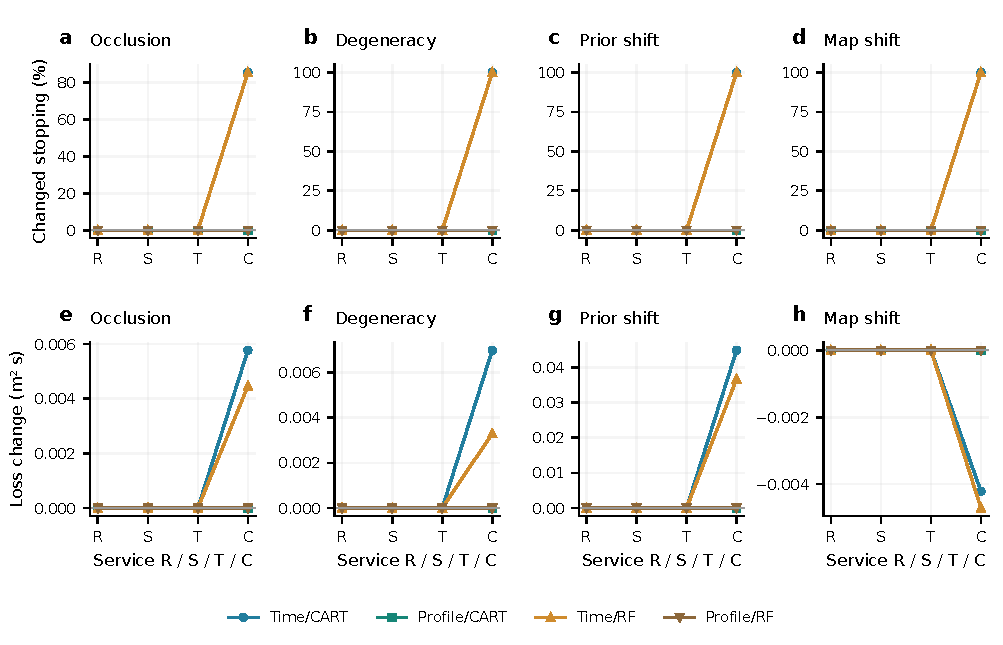
\includegraphics[width=\linewidth]{r8/binding_stress.pdf}
\caption{Binding-constraint stress interventions on all 384 inputs/stratum. R/S/T/C denote the four services. Time screening changes many endpoints under contention and can increase or decrease loss; profile addition remains numerically redundant. These unsupported profiles receive no primary risk card.}\label{fig:stress-ablations}
\end{figure}
\subsection{Integrated CPU and evidence accounting}
\small\begin{longtable}{@{}lllrrrrr@{}}
\caption{Actual Full confirmation. Coverage requires at least one valid issued receipt during execution for each requested event. Dispatch/extra claim columns are microseconds; component and inclusive program ledgers are milliseconds. Inclusive replay contains offline assertion/scoring and is not pure online CPU. Validated Flat has identical numeric/receipt outcomes and its independent CPU rows remain in integrated\_summary.csv.}\label{supp:integrated}\\\toprule
Profile & Service & Task & Coverage & Dispatch $\mu$s & Extra $\mu$s & Component & Inclusive\\\midrule\endfirsthead
\toprule
Profile & Service & Task & Coverage & Dispatch $\mu$s & Extra $\mu$s & Component & Inclusive\\\midrule\endhead
nominal & contended & both\_marginals & 0.000 & 53.0 & 39.4 & 3.512 & 3.551\\
nominal & contended & observation & 0.000 & 44.7 & 32.5 & 3.496 & 3.565\\
nominal & contended & trajectory & 100.000 & 146.2 & 93.1 & 10.683 & 10.776\\
nominal & contended & union & 0.000 & 39.6 & 22.1 & 3.481 & 3.529\\
nominal & relaxed & both\_marginals & 100.000 & 196.2 & 102.8 & 10.349 & 10.395\\
nominal & relaxed & observation & 100.000 & 166.4 & 102.9 & 10.219 & 10.290\\
nominal & relaxed & trajectory & 100.000 & 233.9 & 117.8 & 10.419 & 10.459\\
nominal & relaxed & union & 100.000 & 150.5 & 100.1 & 10.202 & 10.284\\
nominal & standard & both\_marginals & 100.000 & 192.1 & 104.5 & 10.366 & 10.413\\
nominal & standard & observation & 100.000 & 156.6 & 99.7 & 10.289 & 10.369\\
nominal & standard & trajectory & 100.000 & 186.2 & 99.6 & 10.312 & 10.364\\
nominal & standard & union & 100.000 & 145.8 & 100.1 & 10.289 & 10.378\\
nominal & tight & both\_marginals & 0.000 & 29.3 & 22.0 & 3.470 & 3.535\\
nominal & tight & observation & 0.000 & 44.9 & 24.5 & 3.489 & 3.538\\
nominal & tight & trajectory & 0.000 & 72.0 & 32.4 & 3.524 & 3.587\\
nominal & tight & union & 0.000 & 40.7 & 30.1 & 3.490 & 3.533\\
unfitted & contended & both\_marginals & 0.000 & 56.7 & 24.7 & 3.578 & 3.617\\
unfitted & contended & observation & 0.000 & 51.2 & 32.5 & 3.581 & 3.649\\
unfitted & contended & trajectory & 99.951 & 155.4 & 97.0 & 10.700 & 10.787\\
unfitted & contended & union & 0.000 & 43.3 & 23.7 & 3.564 & 3.612\\
unfitted & relaxed & both\_marginals & 99.951 & 209.4 & 108.1 & 10.319 & 10.356\\
unfitted & relaxed & observation & 99.951 & 171.2 & 107.2 & 10.238 & 10.310\\
unfitted & relaxed & trajectory & 99.951 & 224.7 & 122.6 & 10.387 & 10.466\\
unfitted & relaxed & union & 99.951 & 155.4 & 105.5 & 10.225 & 10.305\\
unfitted & standard & both\_marginals & 99.951 & 203.8 & 107.7 & 10.365 & 10.404\\
unfitted & standard & observation & 99.951 & 161.3 & 105.3 & 10.382 & 10.460\\
unfitted & standard & trajectory & 99.951 & 179.6 & 105.2 & 10.320 & 10.375\\
unfitted & standard & union & 99.951 & 156.4 & 104.0 & 10.304 & 10.383\\
unfitted & tight & both\_marginals & 0.000 & 32.1 & 24.2 & 3.553 & 3.621\\
unfitted & tight & observation & 0.000 & 48.0 & 25.9 & 3.571 & 3.625\\
unfitted & tight & trajectory & 0.000 & 70.0 & 32.3 & 3.599 & 3.665\\
unfitted & tight & union & 0.000 & 46.6 & 112.6 & 3.656 & 3.703\\
\bottomrule\end{longtable}\normalsize
\subsection{All complete-route methods and strata}
\small\begin{longtable}{@{}lllrrrrr@{}}
\caption{All twelve live route variants: descriptive means of four matched realizations per geometry/condition. Error units cm; CPU s/600-s route; success \%; no route certificate. Four raw replicate differences per comparison remain in route\_paired\_descriptive.csv.}\label{supp:all-routes}\\\toprule
Geometry & Condition & Method & RMSE & p99 & Success & CPU & Switch\\\midrule\endfirsthead
\toprule
Geometry & Condition & Method & RMSE & p99 & Success & CPU & Switch\\\midrule\endhead
B767 & ordinary & Fixed2 & 3.806 & 9.790 & 97.07 & 2.450 & 0\\
B767 & ordinary & Fixed4 & 3.719 & 9.189 & 94.57 & 3.176 & 0\\
B767 & ordinary & Final & 3.719 & 9.189 & 94.57 & 3.228 & 0\\
B767 & ordinary & FlatCART & 3.706 & 8.875 & 96.49 & 2.711 & 0\\
B767 & ordinary & FlatRF & 3.805 & 9.759 & 97.07 & 2.596 & 0\\
B767 & ordinary & ContractRF & 3.805 & 9.759 & 97.07 & 2.728 & 0\\
B767 & ordinary & OldRAVC & 3.722 & 9.019 & 97.07 & 2.500 & 0\\
B767 & ordinary & KG1 & 3.706 & 8.875 & 96.49 & 2.809 & 0\\
B767 & ordinary & CART\_Time & 3.706 & 8.875 & 96.49 & 2.767 & 0\\
B767 & ordinary & KG1 held & 3.712 & 8.972 & 96.32 & 2.562 & 0\\
B767 & ordinary & Full & 3.715 & 9.036 & 97.24 & 2.514 & 0\\
B767 & ordinary & Validated Flat & 3.715 & 9.036 & 97.24 & 2.504 & 0\\
B767 & contention & Fixed2 & 3.555 & 8.093 & 46.99 & 2.322 & 0\\
B767 & contention & Fixed4 & 3.605 & 8.219 & 45.48 & 2.607 & 0\\
B767 & contention & Final & 3.605 & 8.219 & 45.48 & 2.566 & 0\\
B767 & contention & FlatCART & 3.581 & 8.233 & 54.10 & 2.505 & 0\\
B767 & contention & FlatRF & 3.549 & 8.098 & 44.57 & 2.576 & 0\\
B767 & contention & ContractRF & 3.523 & 8.123 & 44.57 & 2.345 & 0\\
B767 & contention & OldRAVC & 3.550 & 8.095 & 54.85 & 2.299 & 0\\
B767 & contention & KG1 & 3.543 & 8.059 & 54.43 & 2.246 & 0\\
B767 & contention & CART\_Time & 3.543 & 8.059 & 54.43 & 2.038 & 0\\
B767 & contention & KG1 held & 3.545 & 8.065 & 54.43 & 2.325 & 0\\
B767 & contention & Full & 3.531 & 8.090 & 55.02 & 2.019 & 48\\
B767 & contention & Validated Flat & 3.531 & 8.090 & 55.02 & 2.158 & 48\\
B767 & stress & Fixed2 & 8.185 & 15.492 & 42.22 & 2.154 & 0\\
B767 & stress & Fixed4 & 8.215 & 15.547 & 39.97 & 2.557 & 0\\
B767 & stress & Final & 8.215 & 15.547 & 39.97 & 2.668 & 0\\
B767 & stress & FlatCART & 8.215 & 15.581 & 53.85 & 2.583 & 0\\
B767 & stress & FlatRF & 8.187 & 15.514 & 47.41 & 2.450 & 0\\
B767 & stress & ContractRF & 8.186 & 15.537 & 47.74 & 2.136 & 0\\
B767 & stress & OldRAVC & 8.212 & 15.527 & 53.18 & 2.440 & 0\\
B767 & stress & KG1 & 8.200 & 15.384 & 55.85 & 2.207 & 0\\
B767 & stress & CART\_Time & 8.200 & 15.384 & 55.85 & 2.213 & 0\\
B767 & stress & KG1 held & 8.205 & 15.384 & 55.60 & 2.199 & 0\\
B767 & stress & Full & 8.158 & 15.541 & 56.19 & 2.300 & 48\\
B767 & stress & Validated Flat & 8.158 & 15.541 & 56.19 & 2.175 & 48\\
C172 & ordinary & Fixed2 & 4.787 & 10.404 & 94.15 & 2.297 & 0\\
C172 & ordinary & Fixed4 & 4.836 & 11.084 & 91.64 & 3.189 & 0\\
C172 & ordinary & Final & 4.836 & 11.084 & 91.64 & 2.941 & 0\\
C172 & ordinary & FlatCART & 4.832 & 10.478 & 93.06 & 2.378 & 0\\
C172 & ordinary & FlatRF & 4.787 & 10.404 & 94.15 & 2.651 & 0\\
C172 & ordinary & ContractRF & 4.787 & 10.404 & 94.15 & 2.675 & 0\\
C172 & ordinary & OldRAVC & 4.837 & 10.760 & 93.65 & 2.267 & 0\\
C172 & ordinary & KG1 & 4.832 & 10.478 & 93.06 & 2.589 & 0\\
C172 & ordinary & CART\_Time & 4.832 & 10.478 & 93.06 & 2.607 & 0\\
C172 & ordinary & KG1 held & 4.832 & 10.475 & 93.06 & 2.562 & 0\\
C172 & ordinary & Full & 4.805 & 10.436 & 93.81 & 2.518 & 0\\
C172 & ordinary & Validated Flat & 4.805 & 10.436 & 93.81 & 2.491 & 0\\
C172 & contention & Fixed2 & 5.237 & 10.604 & 53.01 & 2.121 & 0\\
C172 & contention & Fixed4 & 5.388 & 11.451 & 51.76 & 2.659 & 0\\
C172 & contention & Final & 5.388 & 11.451 & 51.76 & 2.734 & 0\\
C172 & contention & FlatCART & 5.321 & 10.828 & 81.02 & 2.374 & 0\\
C172 & contention & FlatRF & 5.236 & 10.604 & 53.68 & 2.288 & 0\\
C172 & contention & ContractRF & 5.256 & 10.616 & 53.93 & 2.090 & 0\\
C172 & contention & OldRAVC & 5.193 & 10.582 & 81.77 & 2.173 & 0\\
C172 & contention & KG1 & 5.341 & 10.842 & 80.94 & 2.194 & 0\\
C172 & contention & CART\_Time & 5.341 & 10.842 & 80.94 & 2.162 & 0\\
C172 & contention & KG1 held & 5.342 & 10.843 & 80.85 & 2.096 & 0\\
C172 & contention & Full & 5.234 & 10.569 & 81.61 & 2.028 & 48\\
C172 & contention & Validated Flat & 5.234 & 10.569 & 81.61 & 2.230 & 48\\
C172 & stress & Fixed2 & 14.488 & 28.613 & 10.20 & 2.168 & 0\\
C172 & stress & Fixed4 & 14.333 & 27.971 & 10.03 & 2.545 & 0\\
C172 & stress & Final & 14.333 & 27.971 & 10.03 & 2.754 & 0\\
C172 & stress & FlatCART & 14.494 & 28.595 & 11.62 & 2.432 & 0\\
C172 & stress & FlatRF & 14.490 & 28.606 & 6.19 & 2.285 & 0\\
C172 & stress & ContractRF & 14.398 & 28.363 & 6.27 & 2.342 & 0\\
C172 & stress & OldRAVC & 14.403 & 28.828 & 11.45 & 2.480 & 0\\
C172 & stress & KG1 & 14.439 & 28.348 & 11.45 & 2.198 & 0\\
C172 & stress & CART\_Time & 14.439 & 28.348 & 11.45 & 2.054 & 0\\
C172 & stress & KG1 held & 14.440 & 28.348 & 11.45 & 2.120 & 0\\
C172 & stress & Full & 14.414 & 28.056 & 11.20 & 2.221 & 48\\
C172 & stress & Validated Flat & 14.414 & 28.056 & 11.20 & 2.189 & 48\\
Unfitted & ordinary & Fixed2 & 2.997 & 6.103 & 99.41 & 2.413 & 0\\
Unfitted & ordinary & Fixed4 & 3.022 & 6.256 & 98.91 & 2.688 & 0\\
Unfitted & ordinary & Final & 3.022 & 6.256 & 98.91 & 2.674 & 0\\
Unfitted & ordinary & FlatCART & 3.018 & 6.230 & 99.25 & 2.635 & 0\\
Unfitted & ordinary & FlatRF & 2.997 & 6.103 & 99.41 & 2.521 & 0\\
Unfitted & ordinary & ContractRF & 2.997 & 6.103 & 99.41 & 2.673 & 0\\
Unfitted & ordinary & OldRAVC & 3.006 & 6.137 & 99.25 & 2.290 & 0\\
Unfitted & ordinary & KG1 & 3.018 & 6.230 & 99.25 & 2.618 & 0\\
Unfitted & ordinary & CART\_Time & 3.018 & 6.230 & 99.25 & 2.507 & 0\\
Unfitted & ordinary & KG1 held & 3.027 & 6.255 & 99.16 & 2.577 & 0\\
Unfitted & ordinary & Full & 3.006 & 6.137 & 99.25 & 2.395 & 0\\
Unfitted & ordinary & Validated Flat & 3.006 & 6.137 & 99.25 & 2.235 & 0\\
Unfitted & contention & Fixed2 & 3.064 & 6.134 & 39.21 & 2.108 & 0\\
Unfitted & contention & Fixed4 & 3.071 & 6.206 & 39.21 & 2.353 & 0\\
Unfitted & contention & Final & 3.071 & 6.206 & 39.21 & 2.694 & 0\\
Unfitted & contention & FlatCART & 3.054 & 6.153 & 43.73 & 2.382 & 0\\
Unfitted & contention & FlatRF & 3.057 & 6.111 & 40.22 & 2.322 & 0\\
Unfitted & contention & ContractRF & 2.993 & 5.868 & 40.38 & 2.319 & 0\\
Unfitted & contention & OldRAVC & 3.048 & 6.118 & 43.81 & 2.383 & 0\\
Unfitted & contention & KG1 & 2.993 & 5.903 & 43.65 & 2.078 & 0\\
Unfitted & contention & CART\_Time & 2.993 & 5.903 & 43.65 & 2.027 & 0\\
Unfitted & contention & KG1 held & 2.996 & 5.909 & 43.65 & 1.934 & 0\\
Unfitted & contention & Full & 2.994 & 5.869 & 43.65 & 1.975 & 48\\
Unfitted & contention & Validated Flat & 2.994 & 5.869 & 43.65 & 2.090 & 48\\
Unfitted & stress & Fixed2 & 9.665 & 27.479 & 38.21 & 2.017 & 0\\
Unfitted & stress & Fixed4 & 9.283 & 24.449 & 37.04 & 2.519 & 0\\
Unfitted & stress & Final & 9.283 & 24.449 & 37.04 & 2.531 & 0\\
Unfitted & stress & FlatCART & 9.672 & 27.692 & 45.07 & 2.500 & 0\\
Unfitted & stress & FlatRF & 9.661 & 27.564 & 42.14 & 2.451 & 0\\
Unfitted & stress & ContractRF & 9.633 & 27.118 & 42.56 & 1.907 & 0\\
Unfitted & stress & OldRAVC & 9.269 & 24.467 & 44.82 & 2.464 & 0\\
Unfitted & stress & KG1 & 9.649 & 27.115 & 46.49 & 2.147 & 0\\
Unfitted & stress & CART\_Time & 9.649 & 27.115 & 46.49 & 2.207 & 0\\
Unfitted & stress & KG1 held & 9.654 & 27.115 & 46.49 & 2.042 & 0\\
Unfitted & stress & Full & 9.663 & 27.116 & 45.74 & 2.211 & 48\\
Unfitted & stress & Validated Flat & 9.663 & 27.116 & 45.74 & 2.401 & 48\\
\bottomrule\end{longtable}\normalsize
\subsection{Tail and influence evidence}
\small\begin{longtable}{@{}lllrrrl@{}}
\caption{KG1 influence diagnostics. Gain is baseline minus KG1 ($10^{-3}$ m$^2$s); top-two share is descriptive. I/W/T counts improved/worsened/tied inputs and retains all n=2,048. No top contributor is excluded from primary inference.}\label{supp:influence}\\\toprule
Profile & Service & Baseline & Gain & Top 2 (\%) & Rest gain & I/W/T\\\midrule\endfirsthead
\toprule
Profile & Service & Baseline & Gain & Top 2 (\%) & Rest gain & I/W/T\\\midrule\endhead
geometry & contended & Fixed2 & -1.589 & -22.63 & -1.951 & 851/1194/3\\
geometry & contended & FlatCART & -4.179 & -7.37 & -4.492 & 666/1382/0\\
geometry & contended & FlatRF & -1.830 & -19.66 & -2.192 & 694/1351/3\\
geometry & relaxed & Fixed2 & 2.842 & 8.94 & 2.591 & 1456/515/77\\
geometry & relaxed & FlatCART & 0.000 & -- & 0.000 & 0/0/2048\\
geometry & relaxed & FlatRF & -0.009 & -1137.37 & -0.112 & 277/292/1479\\
geometry & standard & Fixed2 & 2.514 & 10.02 & 2.265 & 458/366/1224\\
geometry & standard & FlatCART & 0.000 & -- & 0.000 & 0/0/2048\\
geometry & standard & FlatRF & 2.512 & 10.03 & 2.262 & 455/365/1228\\
geometry & tight & Fixed2 & -0.004 & -0.00 & -0.004 & 0/7/2041\\
geometry & tight & FlatCART & 0.000 & -- & 0.000 & 0/0/2048\\
geometry & tight & FlatRF & 0.023 & 19.51 & 0.019 & 85/28/1935\\
nominal & contended & Fixed2 & -2.818 & -15.79 & -3.266 & 860/1182/6\\
nominal & contended & FlatCART & -5.094 & -2.11 & -5.206 & 750/1298/0\\
nominal & contended & FlatRF & -3.043 & -14.62 & -3.492 & 779/1263/6\\
nominal & relaxed & Fixed2 & 2.422 & 25.72 & 1.801 & 1202/637/209\\
nominal & relaxed & FlatCART & 0.000 & -- & 0.000 & 0/0/2048\\
nominal & relaxed & FlatRF & -0.283 & -33.03 & -0.377 & 271/292/1485\\
nominal & standard & Fixed2 & 2.169 & 27.99 & 1.563 & 442/374/1232\\
nominal & standard & FlatCART & 0.000 & -- & 0.000 & 0/0/2048\\
nominal & standard & FlatRF & 2.180 & 27.85 & 1.575 & 497/373/1178\\
nominal & tight & Fixed2 & -0.011 & -2.75 & -0.011 & 4/31/2013\\
nominal & tight & FlatCART & 0.000 & -- & 0.000 & 0/0/2048\\
nominal & tight & FlatRF & 0.073 & 5.40 & 0.069 & 372/153/1523\\
\bottomrule\end{longtable}\normalsize
\small\begin{longtable}{@{}llrrrrr@{}}
\caption{Standard-service tails. Loss columns use $10^{-3}$ m$^2$s; error columns cm. Largest-5\% means are descriptive order statistics over every source.}\label{supp:tails}\\\toprule
Profile & Policy & L p95 & L p99 & L top 5\% & Error p99 & Worst error\\\midrule\endfirsthead
\toprule
Profile & Policy & L p95 & L p99 & L top 5\% & Error p99 & Worst error\\\midrule\endhead
nominal & Fixed2 & 47.252 & 105.101 & 95.488 & 16.862 & 52.980\\
nominal & Fixed4 & 37.359 & 76.244 & 65.348 & 14.654 & 25.083\\
nominal & Final & 37.359 & 76.244 & 65.348 & 14.654 & 25.083\\
nominal & FlatCART & 37.550 & 77.893 & 67.486 & 14.654 & 25.083\\
nominal & FlatRF & 47.252 & 105.459 & 95.513 & 16.862 & 52.980\\
nominal & ContractRF & 47.252 & 105.459 & 95.513 & 16.862 & 52.980\\
nominal & OldRAVC & 39.557 & 87.184 & 74.421 & 15.294 & 25.083\\
nominal & KG1 & 37.550 & 77.893 & 67.486 & 14.654 & 25.083\\
unfitted & Fixed2 & 82.222 & 286.196 & 215.495 & 27.364 & 43.740\\
unfitted & Fixed4 & 71.743 & 239.320 & 183.938 & 25.776 & 44.647\\
unfitted & Final & 71.743 & 239.320 & 183.938 & 25.776 & 44.647\\
unfitted & FlatCART & 69.775 & 242.270 & 187.717 & 25.776 & 44.647\\
unfitted & FlatRF & 82.222 & 286.196 & 215.467 & 27.364 & 43.740\\
unfitted & ContractRF & 82.222 & 286.196 & 215.467 & 27.364 & 43.740\\
unfitted & OldRAVC & 72.850 & 246.840 & 190.171 & 26.276 & 44.647\\
unfitted & KG1 & 69.775 & 242.270 & 187.717 & 25.776 & 44.647\\
\bottomrule\end{longtable}\normalsize
\subsection{Audit evidence and retained earlier result displays}
The preflight reports 12 cold-solve equivalence cases, 384 live-prefix/service-budget comparisons, 48 full/procedural equivalence cases and 1,632 constructed fault checks, plus 12 invalid card-schema and five dependency-invalidation fixtures. The final V3 audit covers 16,896 paired pilot contexts and 5,632 first-calibration-chunk policy/service projections, 14 named fault/rollback contexts and entry-point restoration. These software counts are not geometric calibration sample sizes. The real-card audit adds 16 invalid and two valid constructed cases: incorrect attachments 16/4/2/0/0 for no checks/matching/current/history/validated procedural. The normal cases pass all layers. Its deterministic scenario selection supports conformance attribution, not an unbiased field-fault prevalence estimate.

The archive-provider audit reexecutes two complete inputs in both modes. All trace/capture arrays and non-CPU jobs/work/events agree exactly. It adds four executions and zero independent route observations; native CPU differences illustrate archive-boundary contamination rather than a method improvement. Historical metadata checker/dispatcher microbenchmarks retain their original measurement scope and are not combined with current online timing. All review defects, corrections, recovery records and original histories remain in the release.

The following valid R4/R5 experimental displays remain visible with their original populations and timing, separate from new confirmation evidence. Supplied simulation screenshots and all four original physical photos appear in the main paper, with originals retained byte-for-byte.
\begin{figure}[!htbp]\centering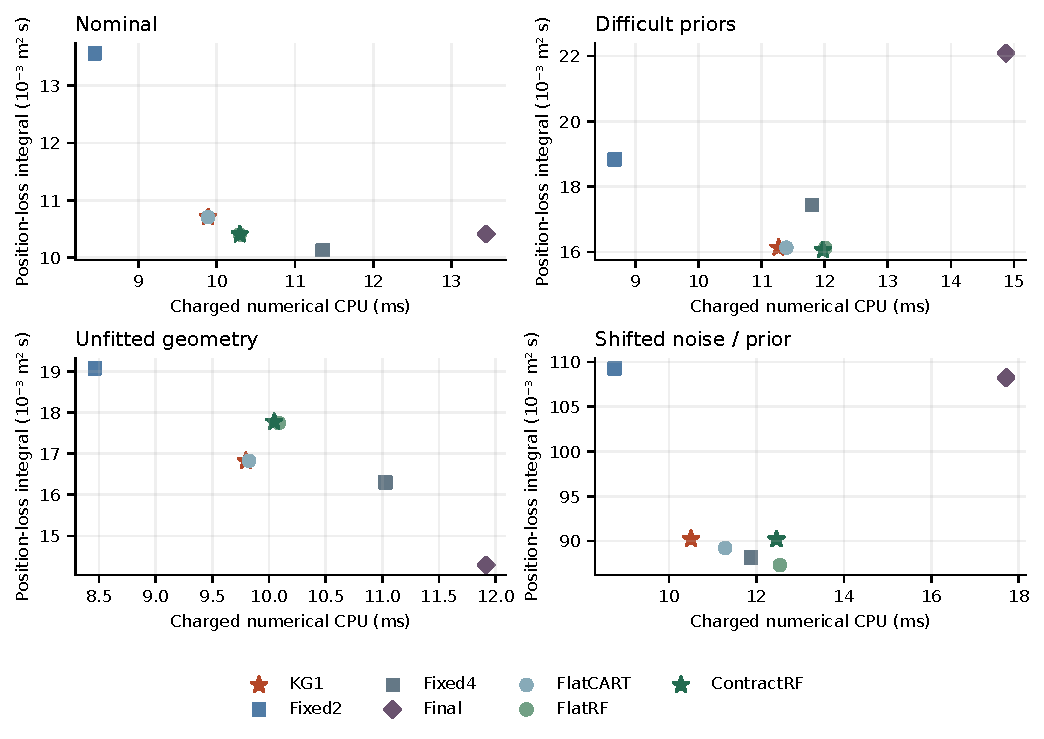
\includegraphics[width=.97\linewidth]{r4/frontier.pdf}\caption{Retained R4 work--loss frontier; Fixed2 and matched Flat controls remain visible.}
\end{figure}
\begin{figure}[!htbp]\centering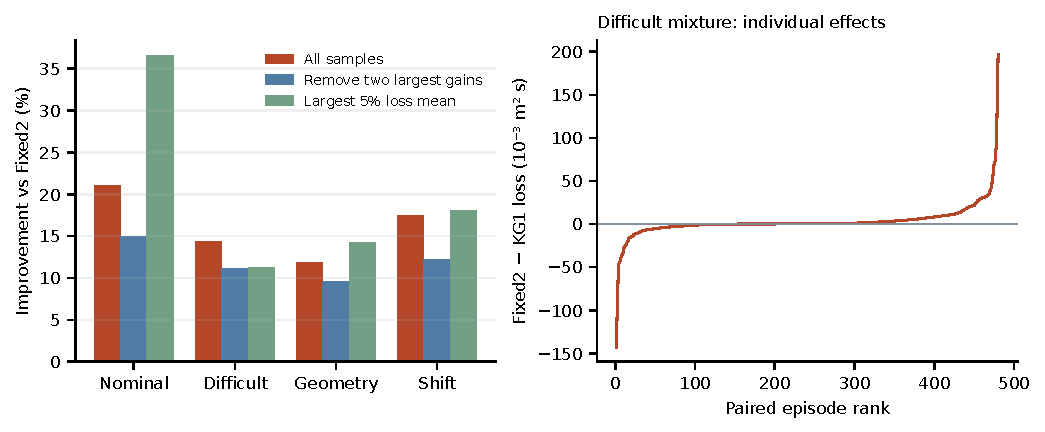
\includegraphics[width=.97\linewidth]{r4/influence.pdf}\caption{Retained R4 influence diagnostic; its contributor concentration is not substituted for R8.}
\end{figure}
\begin{figure}[!htbp]\centering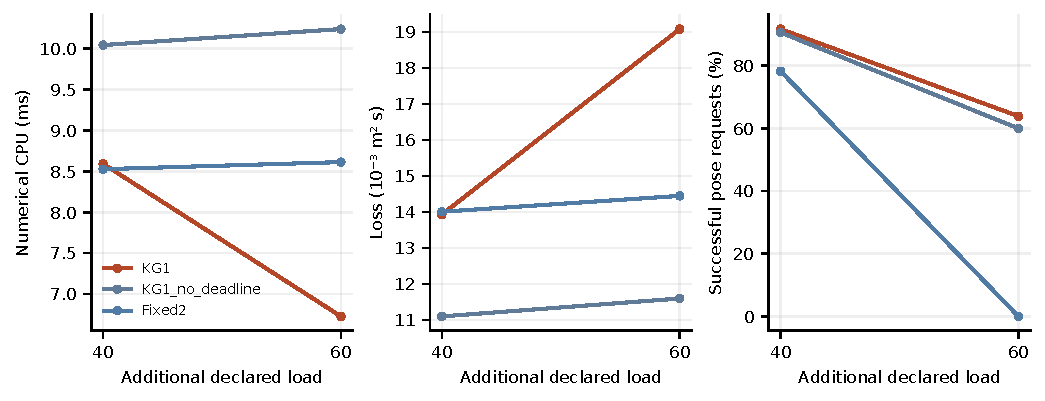
\includegraphics[width=.97\linewidth]{r4/workload.pdf}\caption{Retained R4 unsupported workload results; no old card is transferred to the new service.}
\end{figure}
\begin{figure}[!htbp]\centering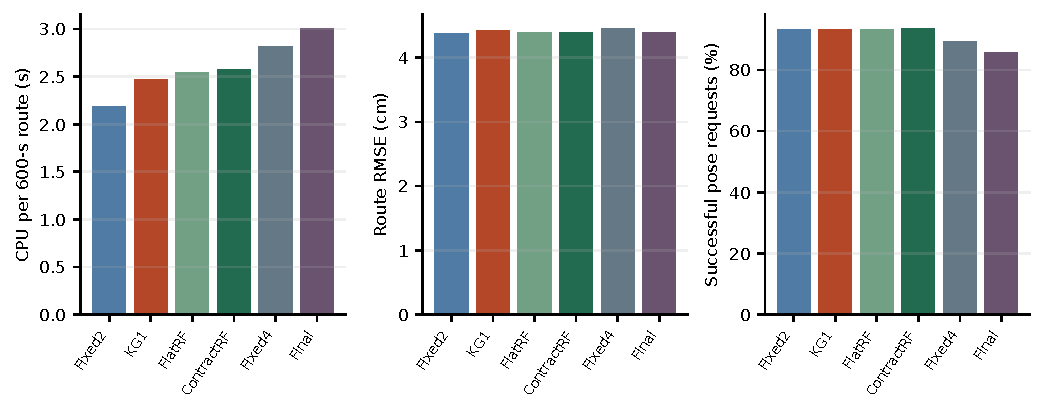
\includegraphics[width=.97\linewidth]{r4/routes.pdf}\caption{Retained R4 nine-input/81-execution complete routes; these are separate from the 36 new inputs.}
\end{figure}
\begin{figure}[!htbp]\centering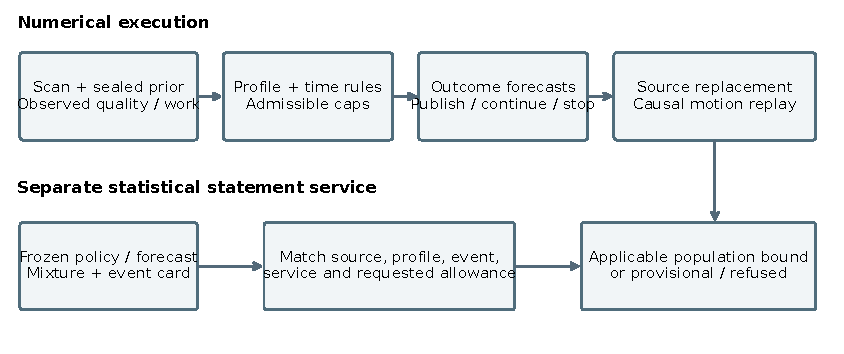
\includegraphics[width=.97\linewidth]{r4/contracts.pdf}\caption{Retained R4 operating-constraint/card comparison with its original finite family.}
\end{figure}
\begin{figure}[!htbp]\centering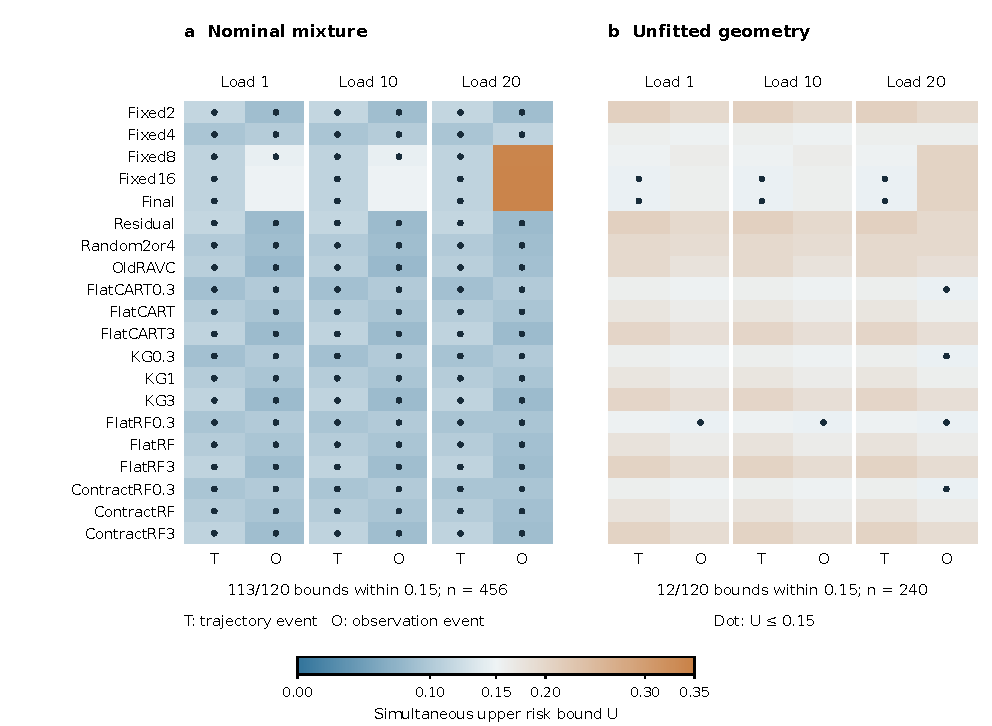
\includegraphics[width=.97\linewidth]{r7/population_cards.pdf}\caption{All 240 retained R4 population cards; separate from the 528 new cards.}
\end{figure}
\begin{figure}[!htbp]\centering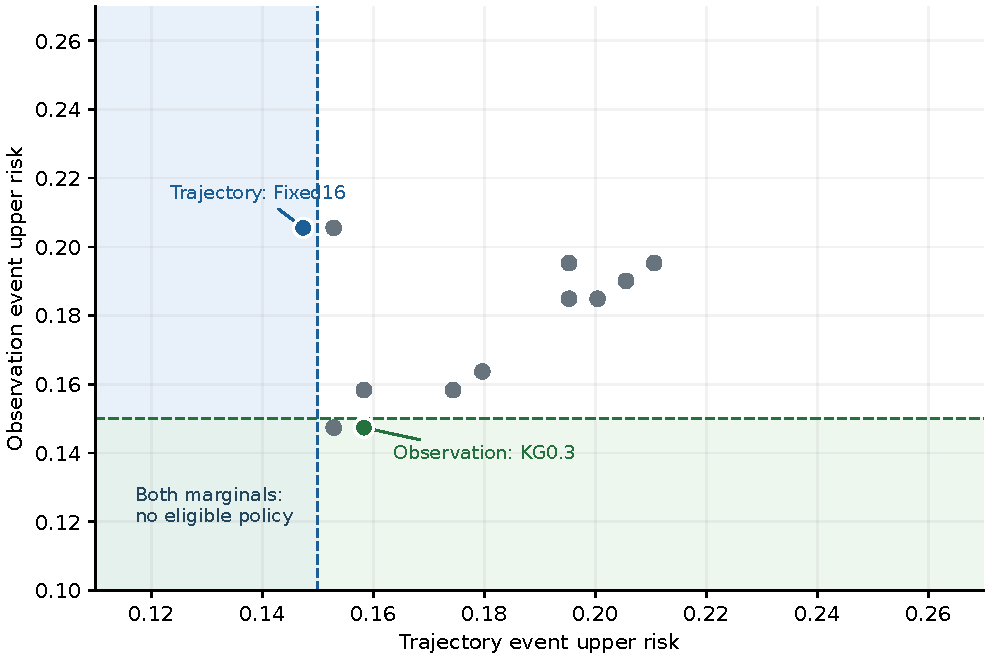
\includegraphics[width=.97\linewidth]{r5/events.pdf}\caption{Retained R5 post-primary event-selection analysis; explicitly secondary rather than new confirmation.}
\end{figure}
\begin{figure}[!htbp]\centering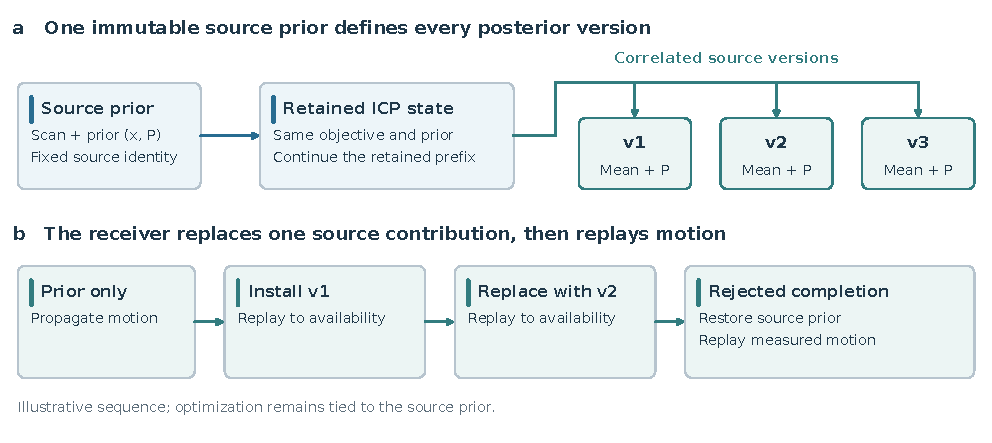
\includegraphics[width=.97\linewidth]{r6/source_versions.pdf}\caption{Retained explanatory source-version replacement and replay interface.}
\end{figure}
\begin{figure}[!htbp]\centering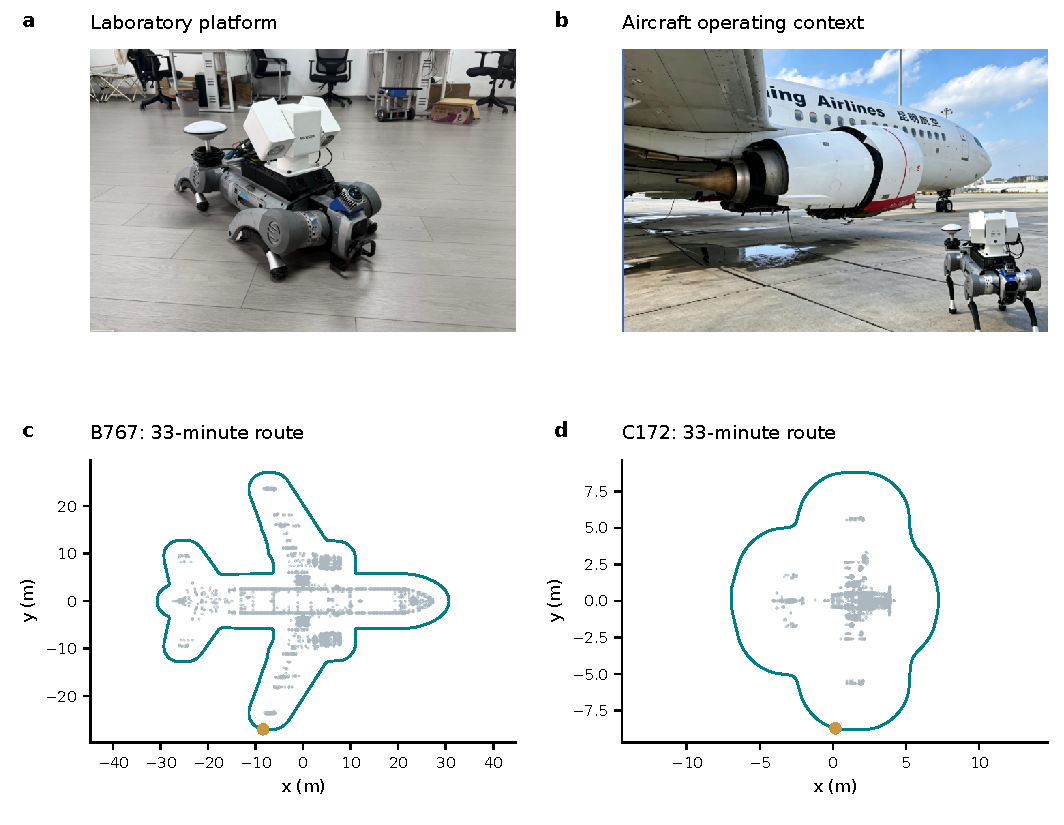
\includegraphics[width=.97\linewidth]{platform_routes.pdf}\caption{Retained original platform photographs and prescribed aircraft route geometry.}
\end{figure}

\FloatBarrier
\section*{Preserved earlier study: distinct inputs, policies, families and timing}

\section{Retained R4 protocol and family records}\label{supp:final}
Final seeds are 5,100,000--5,100,479 (nominal calibration/benchmark), 5,200,000--5,200,639 (nominal confirmation), 5,300,000--5,300,479 (difficult confirmation), 5,400,000--5,400,359 (shift confirmation), 5,500,000--5,500,239 (geometry calibration) and 5,600,000--5,600,479 (geometry confirmation). Benchmark seeds 5,100,000--5,100,023 are excluded from calibration. Ranges are disjoint from fitting, earlier studies and reconstruction pilots.

Tables report the entire 20-policy family. KG is contract-CART; FlatCART/FlatRF omit guards, while ContractRF retains them. Suffix 0.3 or 3 gives price; an omitted suffix means price 1. Residual stops at an eligible second iteration; Random2or4 uses the frozen development continuation frequency. OldRAVC is the earlier frozen policy. Bounds use family size 240 and total confidence error 0.05; allowance 0.15 requires matching event, mixture and service.
\begin{table}[!htbp]\centering\footnotesize
\caption{Nominal calibration at load 1. Event-specific counts and simultaneous upper risks.}\label{supp:calnominal_calibration1}
\begin{tabular}{@{}lrrrrrrr@{}}\toprule
Policy & $n$ & $k_{\rm traj}$ & $U_{\rm traj}$ & $k_{\rm obs}$ & $U_{\rm obs}$ & CPU (ms) & $L$ (m$^2$s)\\\midrule
ContractRF & 456 & 26 & 0.10524 & 23 & 0.09671 & 10.073 & 0.01026\\
ContractRF0.3 & 456 & 23 & 0.09671 & 25 & 0.10241 & 11.702 & 0.00967\\
ContractRF3 & 456 & 29 & 0.11363 & 20 & 0.08802 & 9.195 & 0.01138\\
Final & 456 & 29 & 0.11363 & 43 & 0.15149 & 13.234 & 0.01055\\
Fixed16 & 456 & 29 & 0.11363 & 43 & 0.15149 & 13.234 & 0.01055\\
Fixed2 & 456 & 30 & 0.11640 & 20 & 0.08802 & 8.456 & 0.01154\\
Fixed4 & 456 & 23 & 0.09671 & 26 & 0.10524 & 11.290 & 0.00978\\
Fixed8 & 456 & 29 & 0.11363 & 41 & 0.14619 & 13.162 & 0.01054\\
FlatCART & 456 & 26 & 0.10524 & 23 & 0.09671 & 9.745 & 0.01048\\
FlatCART0.3 & 456 & 21 & 0.09093 & 25 & 0.10241 & 10.700 & 0.00994\\
FlatCART3 & 456 & 29 & 0.11363 & 19 & 0.08508 & 8.839 & 0.01086\\
FlatRF & 456 & 26 & 0.10524 & 23 & 0.09671 & 10.070 & 0.01026\\
FlatRF0.3 & 456 & 23 & 0.09671 & 25 & 0.10241 & 11.693 & 0.00967\\
FlatRF3 & 456 & 29 & 0.11363 & 20 & 0.08802 & 9.190 & 0.01138\\
KG0.3 & 456 & 21 & 0.09093 & 25 & 0.10241 & 10.730 & 0.00994\\
KG1 & 456 & 26 & 0.10524 & 23 & 0.09671 & 9.762 & 0.01048\\
KG3 & 456 & 29 & 0.11363 & 19 & 0.08508 & 8.848 & 0.01086\\
OldRAVC & 456 & 27 & 0.10805 & 18 & 0.08212 & 8.788 & 0.01107\\
Random2or4 & 456 & 25 & 0.10241 & 20 & 0.08802 & 9.796 & 0.01046\\
Residual & 456 & 30 & 0.11640 & 19 & 0.08508 & 8.530 & 0.01153\\
\bottomrule\end{tabular}\end{table}

\begin{table}[!htbp]\centering\footnotesize
\caption{Nominal calibration at load 10. Event-specific counts and simultaneous upper risks.}\label{supp:calnominal_calibration10}
\begin{tabular}{@{}lrrrrrrr@{}}\toprule
Policy & $n$ & $k_{\rm traj}$ & $U_{\rm traj}$ & $k_{\rm obs}$ & $U_{\rm obs}$ & CPU (ms) & $L$ (m$^2$s)\\\midrule
ContractRF & 456 & 26 & 0.10524 & 23 & 0.09671 & 10.169 & 0.01044\\
ContractRF0.3 & 456 & 23 & 0.09671 & 25 & 0.10241 & 11.830 & 0.00986\\
ContractRF3 & 456 & 29 & 0.11363 & 20 & 0.08802 & 9.270 & 0.01153\\
Final & 456 & 29 & 0.11363 & 43 & 0.15149 & 13.301 & 0.01105\\
Fixed16 & 456 & 29 & 0.11363 & 43 & 0.15149 & 13.302 & 0.01105\\
Fixed2 & 456 & 30 & 0.11640 & 20 & 0.08802 & 8.516 & 0.01192\\
Fixed4 & 456 & 23 & 0.09671 & 26 & 0.10524 & 11.359 & 0.01028\\
Fixed8 & 456 & 29 & 0.11363 & 41 & 0.14619 & 13.229 & 0.01103\\
FlatCART & 456 & 26 & 0.10524 & 23 & 0.09671 & 9.837 & 0.01065\\
FlatCART0.3 & 456 & 21 & 0.09093 & 25 & 0.10241 & 10.813 & 0.01013\\
FlatCART3 & 456 & 29 & 0.11363 & 19 & 0.08508 & 8.911 & 0.01102\\
FlatRF & 456 & 26 & 0.10524 & 23 & 0.09671 & 10.163 & 0.01044\\
FlatRF0.3 & 456 & 23 & 0.09671 & 25 & 0.10241 & 11.822 & 0.00986\\
FlatRF3 & 456 & 29 & 0.11363 & 20 & 0.08802 & 9.263 & 0.01153\\
KG0.3 & 456 & 21 & 0.09093 & 25 & 0.10241 & 10.822 & 0.01013\\
KG1 & 456 & 26 & 0.10524 & 23 & 0.09671 & 9.847 & 0.01065\\
KG3 & 456 & 29 & 0.11363 & 19 & 0.08508 & 8.918 & 0.01102\\
OldRAVC & 456 & 27 & 0.10805 & 18 & 0.08212 & 8.854 & 0.01128\\
Random2or4 & 456 & 25 & 0.10241 & 20 & 0.08802 & 9.858 & 0.01088\\
Residual & 456 & 30 & 0.11640 & 19 & 0.08508 & 8.596 & 0.01167\\
\bottomrule\end{tabular}\end{table}

\begin{table}[!htbp]\centering\footnotesize
\caption{Nominal calibration at load 20. Event-specific counts and simultaneous upper risks.}\label{supp:calnominal_calibration20}
\begin{tabular}{@{}lrrrrrrr@{}}\toprule
Policy & $n$ & $k_{\rm traj}$ & $U_{\rm traj}$ & $k_{\rm obs}$ & $U_{\rm obs}$ & CPU (ms) & $L$ (m$^2$s)\\\midrule
ContractRF & 456 & 26 & 0.10524 & 21 & 0.09093 & 10.231 & 0.01079\\
ContractRF0.3 & 456 & 23 & 0.09671 & 23 & 0.09671 & 11.848 & 0.01023\\
ContractRF3 & 456 & 29 & 0.11363 & 20 & 0.08802 & 9.329 & 0.01186\\
Final & 456 & 29 & 0.11363 & 121 & 0.34343 & 13.372 & 0.01162\\
Fixed16 & 456 & 29 & 0.11363 & 121 & 0.34343 & 13.371 & 0.01162\\
Fixed2 & 456 & 30 & 0.11640 & 20 & 0.08802 & 8.527 & 0.01201\\
Fixed4 & 456 & 23 & 0.09671 & 29 & 0.11363 & 11.420 & 0.01074\\
Fixed8 & 456 & 29 & 0.11363 & 120 & 0.34109 & 13.299 & 0.01161\\
FlatCART & 456 & 26 & 0.10524 & 23 & 0.09671 & 9.932 & 0.01100\\
FlatCART0.3 & 456 & 21 & 0.09093 & 25 & 0.10241 & 10.932 & 0.01048\\
FlatCART3 & 456 & 29 & 0.11363 & 19 & 0.08508 & 8.985 & 0.01136\\
FlatRF & 456 & 26 & 0.10524 & 21 & 0.09093 & 10.250 & 0.01078\\
FlatRF0.3 & 456 & 23 & 0.09671 & 23 & 0.09671 & 11.946 & 0.01022\\
FlatRF3 & 456 & 29 & 0.11363 & 20 & 0.08802 & 9.336 & 0.01185\\
KG0.3 & 456 & 22 & 0.09383 & 25 & 0.10241 & 10.867 & 0.01055\\
KG1 & 456 & 26 & 0.10524 & 23 & 0.09671 & 9.930 & 0.01100\\
KG3 & 456 & 29 & 0.11363 & 19 & 0.08508 & 8.980 & 0.01136\\
OldRAVC & 456 & 27 & 0.10805 & 21 & 0.09093 & 8.918 & 0.01162\\
Random2or4 & 456 & 25 & 0.10241 & 20 & 0.08802 & 9.895 & 0.01115\\
Residual & 456 & 30 & 0.11640 & 19 & 0.08508 & 8.670 & 0.01199\\
\bottomrule\end{tabular}\end{table}

\begin{table}[!htbp]\centering\footnotesize
\caption{Procedural geometry calibration at load 1. Event-specific counts and simultaneous upper risks.}\label{supp:calgeometry_calibration1}
\begin{tabular}{@{}lrrrrrrr@{}}\toprule
Policy & $n$ & $k_{\rm traj}$ & $U_{\rm traj}$ & $k_{\rm obs}$ & $U_{\rm obs}$ & CPU (ms) & $L$ (m$^2$s)\\\midrule
ContractRF & 240 & 23 & 0.17966 & 20 & 0.16372 & 9.728 & 0.01871\\
ContractRF0.3 & 240 & 19 & 0.15832 & 18 & 0.15288 & 10.734 & 0.01778\\
ContractRF3 & 240 & 28 & 0.20554 & 25 & 0.19011 & 8.912 & 0.02099\\
Final & 240 & 17 & 0.14739 & 19 & 0.15832 & 11.572 & 0.01597\\
Fixed16 & 240 & 17 & 0.14739 & 19 & 0.15832 & 11.572 & 0.01597\\
Fixed2 & 240 & 29 & 0.21063 & 26 & 0.19528 & 8.223 & 0.02142\\
Fixed4 & 240 & 19 & 0.15832 & 18 & 0.15288 & 10.727 & 0.01779\\
Fixed8 & 240 & 18 & 0.15288 & 20 & 0.16372 & 11.484 & 0.01629\\
FlatCART & 240 & 22 & 0.17438 & 20 & 0.16372 & 9.568 & 0.01862\\
FlatCART0.3 & 240 & 19 & 0.15832 & 18 & 0.15288 & 9.975 & 0.01792\\
FlatCART3 & 240 & 27 & 0.20042 & 24 & 0.18490 & 8.642 & 0.02015\\
FlatRF & 240 & 23 & 0.17966 & 20 & 0.16372 & 9.749 & 0.01871\\
FlatRF0.3 & 240 & 18 & 0.15288 & 17 & 0.14739 & 10.882 & 0.01694\\
FlatRF3 & 240 & 28 & 0.20554 & 25 & 0.19011 & 8.927 & 0.02099\\
KG0.3 & 240 & 19 & 0.15832 & 18 & 0.15288 & 9.909 & 0.01801\\
KG1 & 240 & 22 & 0.17438 & 20 & 0.16372 & 9.557 & 0.01862\\
KG3 & 240 & 27 & 0.20042 & 24 & 0.18490 & 8.625 & 0.02015\\
OldRAVC & 240 & 26 & 0.19528 & 23 & 0.17966 & 8.559 & 0.01949\\
Random2or4 & 240 & 26 & 0.19528 & 25 & 0.19011 & 9.412 & 0.02070\\
Residual & 240 & 29 & 0.21063 & 26 & 0.19528 & 8.292 & 0.02142\\
\bottomrule\end{tabular}\end{table}

\begin{table}[!htbp]\centering\footnotesize
\caption{Procedural geometry calibration at load 10. Event-specific counts and simultaneous upper risks.}\label{supp:calgeometry_calibration10}
\begin{tabular}{@{}lrrrrrrr@{}}\toprule
Policy & $n$ & $k_{\rm traj}$ & $U_{\rm traj}$ & $k_{\rm obs}$ & $U_{\rm obs}$ & CPU (ms) & $L$ (m$^2$s)\\\midrule
ContractRF & 240 & 23 & 0.17966 & 20 & 0.16372 & 9.822 & 0.01876\\
ContractRF0.3 & 240 & 19 & 0.15832 & 18 & 0.15288 & 10.848 & 0.01786\\
ContractRF3 & 240 & 28 & 0.20554 & 25 & 0.19011 & 8.984 & 0.02099\\
Final & 240 & 17 & 0.14739 & 19 & 0.15832 & 11.641 & 0.01622\\
Fixed16 & 240 & 17 & 0.14739 & 19 & 0.15832 & 11.641 & 0.01622\\
Fixed2 & 240 & 29 & 0.21063 & 26 & 0.19528 & 8.278 & 0.02147\\
Fixed4 & 240 & 19 & 0.15832 & 18 & 0.15288 & 10.796 & 0.01798\\
Fixed8 & 240 & 18 & 0.15288 & 20 & 0.16372 & 11.552 & 0.01651\\
FlatCART & 240 & 22 & 0.17438 & 20 & 0.16372 & 9.661 & 0.01867\\
FlatCART0.3 & 240 & 19 & 0.15832 & 18 & 0.15288 & 10.077 & 0.01800\\
FlatCART3 & 240 & 27 & 0.20042 & 24 & 0.18490 & 8.713 & 0.02017\\
FlatRF & 240 & 23 & 0.17966 & 20 & 0.16372 & 9.840 & 0.01876\\
FlatRF0.3 & 240 & 18 & 0.15288 & 17 & 0.14739 & 10.999 & 0.01703\\
FlatRF3 & 240 & 28 & 0.20554 & 25 & 0.19011 & 9.001 & 0.02099\\
KG0.3 & 240 & 19 & 0.15832 & 18 & 0.15288 & 9.988 & 0.01808\\
KG1 & 240 & 22 & 0.17438 & 20 & 0.16372 & 9.640 & 0.01868\\
KG3 & 240 & 27 & 0.20042 & 24 & 0.18490 & 8.694 & 0.02017\\
OldRAVC & 240 & 26 & 0.19528 & 23 & 0.17966 & 8.620 & 0.01948\\
Random2or4 & 240 & 26 & 0.19528 & 25 & 0.19011 & 9.472 & 0.02079\\
Residual & 240 & 29 & 0.21063 & 26 & 0.19528 & 8.355 & 0.02143\\
\bottomrule\end{tabular}\end{table}

\begin{table}[!htbp]\centering\footnotesize
\caption{Procedural geometry calibration at load 20. Event-specific counts and simultaneous upper risks.}\label{supp:calgeometry_calibration20}
\begin{tabular}{@{}lrrrrrrr@{}}\toprule
Policy & $n$ & $k_{\rm traj}$ & $U_{\rm traj}$ & $k_{\rm obs}$ & $U_{\rm obs}$ & CPU (ms) & $L$ (m$^2$s)\\\midrule
ContractRF & 240 & 23 & 0.17966 & 20 & 0.16372 & 9.910 & 0.01894\\
ContractRF0.3 & 240 & 19 & 0.15832 & 17 & 0.14739 & 10.960 & 0.01806\\
ContractRF3 & 240 & 28 & 0.20554 & 25 & 0.19011 & 9.058 & 0.02111\\
Final & 240 & 17 & 0.14739 & 28 & 0.20554 & 11.694 & 0.01639\\
Fixed16 & 240 & 17 & 0.14739 & 28 & 0.20554 & 11.693 & 0.01639\\
Fixed2 & 240 & 29 & 0.21063 & 26 & 0.19528 & 8.294 & 0.02153\\
Fixed4 & 240 & 19 & 0.15832 & 19 & 0.15832 & 10.845 & 0.01808\\
Fixed8 & 240 & 18 & 0.15288 & 28 & 0.20554 & 11.604 & 0.01667\\
FlatCART & 240 & 22 & 0.17438 & 19 & 0.15832 & 9.765 & 0.01885\\
FlatCART0.3 & 240 & 19 & 0.15832 & 17 & 0.14739 & 10.186 & 0.01819\\
FlatCART3 & 240 & 27 & 0.20042 & 24 & 0.18490 & 8.793 & 0.02031\\
FlatRF & 240 & 23 & 0.17966 & 20 & 0.16372 & 9.929 & 0.01894\\
FlatRF0.3 & 240 & 18 & 0.15288 & 17 & 0.14739 & 11.115 & 0.01727\\
FlatRF3 & 240 & 28 & 0.20554 & 25 & 0.19011 & 9.075 & 0.02111\\
KG0.3 & 240 & 19 & 0.15832 & 17 & 0.14739 & 10.098 & 0.01828\\
KG1 & 240 & 22 & 0.17438 & 19 & 0.15832 & 9.745 & 0.01885\\
KG3 & 240 & 27 & 0.20042 & 24 & 0.18490 & 8.777 & 0.02031\\
OldRAVC & 240 & 26 & 0.19528 & 24 & 0.18490 & 8.690 & 0.01961\\
Random2or4 & 240 & 26 & 0.19528 & 26 & 0.19528 & 9.506 & 0.02085\\
Residual & 240 & 29 & 0.21063 & 26 & 0.19528 & 8.434 & 0.02152\\
\bottomrule\end{tabular}\end{table}

\FloatBarrier
\section{All-family independent confirmation}
Tables include all 20 calibrated policies. Each cell is numerical CPU (ms) / loss (m$^2$s) / trajectory failures / observation successes. Loads reuse the same inputs and are not additional independent samples.
\begin{table}[!htbp]\centering\scriptsize
\caption{Nominal: $n=640$ independent inputs.}\label{supp:confirmnominal_confirmation}
\begin{tabular}{@{}lrrr@{}}\toprule
Policy & Load 1 & Load 10 & Load 20\\\midrule
ContractRF & 10.12/0.00987/24/621 & 10.22/0.01008/24/621 & 10.30/0.01040/24/621\\
ContractRF0.3 & 11.82/0.00853/20/617 & 11.95/0.00878/20/617 & 11.91/0.00947/21/618\\
ContractRF3 & 9.28/0.01126/35/611 & 9.36/0.01143/35/611 & 9.42/0.01172/35/610\\
Final & 13.31/0.00932/30/581 & 13.37/0.00984/30/581 & 13.44/0.01041/30/466\\
Fixed16 & 13.31/0.00932/30/581 & 13.37/0.00984/30/581 & 13.44/0.01041/30/466\\
Fixed2 & 8.37/0.01319/46/600 & 8.43/0.01350/46/600 & 8.44/0.01357/46/600\\
Fixed4 & 11.23/0.00923/25/603 & 11.29/0.00970/25/603 & 11.35/0.01013/25/597\\
Fixed8 & 13.17/0.00928/30/583 & 13.24/0.00977/30/583 & 13.31/0.01034/30/474\\
FlatCART & 9.70/0.01019/29/617 & 9.79/0.01038/29/617 & 9.89/0.01070/29/617\\
FlatCART0.3 & 10.74/0.00901/23/611 & 10.86/0.00923/23/611 & 10.98/0.00958/23/615\\
FlatCART3 & 8.80/0.01107/32/614 & 8.87/0.01124/32/614 & 8.94/0.01154/32/614\\
FlatRF & 10.11/0.00987/24/621 & 10.21/0.01008/24/621 & 10.30/0.01040/24/620\\
FlatRF0.3 & 11.81/0.00853/20/617 & 11.94/0.00878/20/617 & 12.07/0.00914/20/617\\
FlatRF3 & 9.27/0.01126/35/611 & 9.34/0.01143/35/611 & 9.41/0.01172/35/610\\
KG0.3 & 10.78/0.00901/23/611 & 10.86/0.00923/23/611 & 10.92/0.00956/22/615\\
KG1 & 9.72/0.01019/29/617 & 9.80/0.01038/29/617 & 9.89/0.01070/29/617\\
KG3 & 8.81/0.01107/32/614 & 8.87/0.01124/32/614 & 8.95/0.01154/32/614\\
OldRAVC & 8.86/0.01178/35/610 & 8.92/0.01199/35/610 & 9.00/0.01230/35/605\\
Random2or4 & 9.62/0.01086/32/605 & 9.68/0.01126/32/605 & 9.71/0.01147/32/604\\
Residual & 8.45/0.01312/45/602 & 8.51/0.01325/45/602 & 8.59/0.01349/45/602\\
\bottomrule\end{tabular}\end{table}

\begin{table}[!htbp]\centering\scriptsize
\caption{Difficult priors: $n=480$ independent inputs.}\label{supp:confirmdifficult_confirmation}
\begin{tabular}{@{}lrrr@{}}\toprule
Policy & Load 1 & Load 10 & Load 20\\\midrule
ContractRF & 11.76/0.01459/55/435 & 11.88/0.01513/55/435 & 11.97/0.01605/55/438\\
ContractRF0.3 & 12.72/0.01406/54/434 & 12.86/0.01461/54/434 & 12.86/0.01600/56/435\\
ContractRF3 & 9.79/0.01510/53/438 & 9.88/0.01562/53/438 & 9.95/0.01661/53/438\\
Final & 14.72/0.01870/69/406 & 14.79/0.02027/69/406 & 14.87/0.02208/70/266\\
Fixed16 & 14.72/0.01870/69/406 & 14.79/0.02027/69/406 & 14.87/0.02208/70/266\\
Fixed2 & 8.60/0.01740/67/425 & 8.67/0.01870/67/425 & 8.67/0.01883/67/424\\
Fixed4 & 11.66/0.01455/57/432 & 11.73/0.01600/57/432 & 11.80/0.01743/57/426\\
Fixed8 & 14.44/0.01787/68/408 & 14.51/0.01934/68/408 & 14.59/0.02121/68/269\\
FlatCART & 11.15/0.01461/54/437 & 11.27/0.01509/54/437 & 11.39/0.01613/54/437\\
FlatCART0.3 & 11.60/0.01432/53/433 & 11.73/0.01482/53/433 & 11.86/0.01586/53/436\\
FlatCART3 & 9.57/0.01549/59/435 & 9.66/0.01596/59/435 & 9.75/0.01697/59/435\\
FlatRF & 11.77/0.01459/55/435 & 11.89/0.01513/55/435 & 12.01/0.01612/55/437\\
FlatRF0.3 & 12.86/0.01395/54/433 & 13.00/0.01450/54/433 & 13.14/0.01552/54/435\\
FlatRF3 & 9.80/0.01510/53/438 & 9.88/0.01563/53/438 & 9.96/0.01661/53/438\\
KG0.3 & 11.35/0.01451/54/436 & 11.45/0.01499/54/436 & 11.49/0.01607/54/436\\
KG1 & 11.06/0.01463/54/437 & 11.17/0.01511/54/437 & 11.27/0.01613/54/437\\
KG3 & 9.50/0.01549/59/435 & 9.58/0.01595/59/435 & 9.66/0.01696/59/435\\
OldRAVC & 9.58/0.01560/54/438 & 9.65/0.01658/54/438 & 9.70/0.01761/54/425\\
Random2or4 & 10.05/0.01541/67/427 & 10.11/0.01678/67/427 & 10.15/0.01757/67/424\\
Residual & 8.68/0.01690/66/427 & 8.75/0.01730/66/427 & 8.82/0.01830/66/427\\
\bottomrule\end{tabular}\end{table}

\begin{table}[!htbp]\centering\scriptsize
\caption{Unfitted geometry: $n=480$ independent inputs.}\label{supp:confirmgeometry_confirmation}
\begin{tabular}{@{}lrrr@{}}\toprule
Policy & Load 1 & Load 10 & Load 20\\\midrule
ContractRF & 9.89/0.01738/55/434 & 9.98/0.01748/55/434 & 10.05/0.01777/55/432\\
ContractRF0.3 & 10.91/0.01605/48/436 & 11.02/0.01618/48/436 & 11.10/0.01654/48/434\\
ContractRF3 & 9.08/0.01817/56/434 & 9.16/0.01825/56/434 & 9.23/0.01849/56/433\\
Final & 11.79/0.01346/37/440 & 11.86/0.01390/37/440 & 11.92/0.01429/37/407\\
Fixed16 & 11.79/0.01346/37/440 & 11.86/0.01390/37/440 & 11.92/0.01429/37/407\\
Fixed2 & 8.39/0.01877/57/433 & 8.45/0.01900/57/433 & 8.46/0.01907/57/433\\
Fixed4 & 10.91/0.01565/49/435 & 10.97/0.01601/49/435 & 11.03/0.01630/49/430\\
Fixed8 & 11.76/0.01355/38/440 & 11.83/0.01398/38/440 & 11.89/0.01438/38/408\\
FlatCART & 9.63/0.01641/52/436 & 9.72/0.01654/52/436 & 9.82/0.01682/52/435\\
FlatCART0.3 & 10.13/0.01575/45/439 & 10.24/0.01589/45/439 & 10.35/0.01620/45/436\\
FlatCART3 & 8.79/0.01794/58/431 & 8.87/0.01803/58/431 & 8.94/0.01828/58/431\\
FlatRF & 9.91/0.01738/55/434 & 9.99/0.01748/55/434 & 10.09/0.01774/55/432\\
FlatRF0.3 & 11.02/0.01567/46/437 & 11.13/0.01581/46/437 & 11.25/0.01613/46/434\\
FlatRF3 & 9.10/0.01817/56/434 & 9.17/0.01825/56/434 & 9.25/0.01849/56/433\\
KG0.3 & 10.01/0.01613/49/437 & 10.10/0.01626/49/437 & 10.19/0.01656/49/436\\
KG1 & 9.62/0.01641/52/436 & 9.71/0.01654/52/436 & 9.80/0.01682/52/435\\
KG3 & 8.78/0.01794/58/431 & 8.85/0.01803/58/431 & 8.92/0.01828/58/431\\
OldRAVC & 8.80/0.01733/54/436 & 8.87/0.01744/54/436 & 8.94/0.01772/54/434\\
Random2or4 & 9.58/0.01688/52/436 & 9.64/0.01717/52/436 & 9.67/0.01733/52/432\\
Residual & 8.46/0.01877/57/433 & 8.53/0.01884/57/433 & 8.60/0.01907/57/433\\
\bottomrule\end{tabular}\end{table}

\begin{table}[!htbp]\centering\scriptsize
\caption{Shifted noise/prior: $n=360$ independent inputs.}\label{supp:confirmshift_confirmation}
\begin{tabular}{@{}lrrr@{}}\toprule
Policy & Load 1 & Load 10 & Load 20\\\midrule
ContractRF & 12.36/0.08499/197/151 & 12.44/0.08619/197/151 & 12.46/0.09018/198/154\\
ContractRF0.3 & 12.55/0.08499/197/151 & 12.63/0.08619/197/151 & 12.64/0.09017/198/154\\
ContractRF3 & 11.33/0.08415/195/152 & 11.39/0.08537/195/152 & 11.39/0.08938/196/152\\
Final & 17.62/0.10503/217/117 & 17.67/0.10668/217/115 & 17.71/0.10826/220/40\\
Fixed16 & 17.62/0.10503/217/117 & 17.67/0.10668/217/115 & 17.71/0.10826/220/40\\
Fixed2 & 8.72/0.10826/204/138 & 8.75/0.10923/204/138 & 8.76/0.10930/204/138\\
Fixed4 & 11.79/0.08499/197/151 & 11.83/0.08659/197/151 & 11.87/0.08815/197/150\\
Fixed8 & 16.63/0.09825/208/128 & 16.67/0.09992/208/128 & 16.73/0.10182/208/44\\
FlatCART & 11.16/0.08717/196/151 & 11.23/0.08821/196/151 & 11.28/0.08921/196/150\\
FlatCART0.3 & 11.17/0.08717/196/151 & 11.23/0.08821/196/151 & 11.28/0.08920/196/150\\
FlatCART3 & 10.47/0.08727/195/147 & 10.53/0.08830/195/147 & 10.57/0.08929/195/146\\
FlatRF & 12.39/0.08499/197/151 & 12.47/0.08619/197/151 & 12.54/0.08730/197/154\\
FlatRF0.3 & 12.63/0.08499/197/151 & 12.71/0.08619/197/151 & 12.78/0.08730/197/154\\
FlatRF3 & 11.35/0.08415/195/152 & 11.42/0.08537/195/152 & 11.47/0.08651/195/152\\
KG0.3 & 10.44/0.08562/196/150 & 10.48/0.08676/196/150 & 10.50/0.09021/197/149\\
KG1 & 10.43/0.08562/196/150 & 10.48/0.08675/196/150 & 10.50/0.09021/197/149\\
KG3 & 9.81/0.08569/195/146 & 9.86/0.08683/195/146 & 9.88/0.09028/196/145\\
OldRAVC & 17.60/0.10508/218/117 & 17.64/0.10673/218/115 & 17.69/0.10829/221/43\\
Random2or4 & 10.13/0.09422/203/143 & 10.16/0.09555/203/143 & 10.18/0.09642/203/143\\
Residual & 12.50/0.07913/187/168 & 12.55/0.08048/187/168 & 12.58/0.08174/187/160\\
\bottomrule\end{tabular}\end{table}

\FloatBarrier
\section{Complete routes and additional workload}
Route seeds are 5,700,000 + replicate + 10,000 $\times$ geometry index (B767: 0; C172: 1; procedural: 2), with replicate 0, 1 or 2. Each raw input is shared by nine variants. Each route has 299 observation opportunities. Means below use three seeds per geometry.
\begin{table}[!htbp]\centering\footnotesize
\caption{B767 means over three independent 600-s routes.}\label{supp:routeB767}
\begin{tabular}{@{}lrrrrr@{}}\toprule
Policy & CPU (s) & RMSE (cm) & $L$ (m$^2$s) & Ready (\%) & Success (\%)\\\midrule
ContractRF & 2.654 & 3.962 & 1.0650 & 97.77 & 96.10\\
Final & 3.231 & 3.860 & 1.0088 & 84.17 & 82.83\\
Fixed2 & 2.249 & 3.968 & 1.0515 & 97.55 & 95.65\\
Fixed4 & 3.054 & 3.971 & 1.0640 & 91.30 & 89.86\\
FlatRF & 2.627 & 3.963 & 1.0652 & 97.77 & 96.21\\
KG1 & 2.664 & 4.000 & 1.0713 & 97.66 & 96.10\\
KG1 held & 2.876 & 3.976 & 1.0656 & 95.09 & 93.53\\
KG1 w/o time & 2.645 & 4.001 & 1.0717 & 97.44 & 95.88\\
KG1 w/o profile & 2.645 & 4.001 & 1.0717 & 97.32 & 95.76\\
\bottomrule\end{tabular}\end{table}

\begin{table}[!htbp]\centering\footnotesize
\caption{C172 means over three independent 600-s routes.}\label{supp:routeC172}
\begin{tabular}{@{}lrrrrr@{}}\toprule
Policy & CPU (s) & RMSE (cm) & $L$ (m$^2$s) & Ready (\%) & Success (\%)\\\midrule
ContractRF & 2.527 & 5.272 & 2.0817 & 98.44 & 89.19\\
Final & 3.035 & 5.199 & 2.0319 & 89.30 & 82.16\\
Fixed2 & 2.232 & 5.223 & 2.0324 & 98.22 & 89.19\\
Fixed4 & 2.711 & 5.287 & 2.1030 & 95.54 & 86.29\\
FlatRF & 2.511 & 5.269 & 2.0793 & 98.33 & 89.19\\
KG1 & 2.262 & 5.276 & 2.0780 & 98.66 & 89.19\\
KG1 held & 2.294 & 5.276 & 2.0780 & 98.55 & 89.07\\
KG1 w/o time & 2.489 & 5.276 & 2.0784 & 98.55 & 89.19\\
KG1 w/o profile & 2.361 & 5.276 & 2.0781 & 98.77 & 89.30\\
\bottomrule\end{tabular}\end{table}

\begin{table}[!htbp]\centering\footnotesize
\caption{Procedural means over three independent 600-s routes.}\label{supp:routeProceduralAirframe}
\begin{tabular}{@{}lrrrrr@{}}\toprule
Policy & CPU (s) & RMSE (cm) & $L$ (m$^2$s) & Ready (\%) & Success (\%)\\\midrule
ContractRF & 2.534 & 3.932 & 1.2043 & 99.22 & 94.98\\
Final & 2.738 & 4.127 & 1.3283 & 96.43 & 92.08\\
Fixed2 & 2.070 & 3.921 & 1.1967 & 99.22 & 94.98\\
Fixed4 & 2.701 & 4.080 & 1.3075 & 96.32 & 91.97\\
FlatRF & 2.499 & 3.932 & 1.2043 & 99.00 & 94.76\\
KG1 & 2.491 & 3.983 & 1.2383 & 98.44 & 94.31\\
KG1 held & 2.434 & 3.991 & 1.2430 & 98.22 & 94.09\\
KG1 w/o time & 2.391 & 3.983 & 1.2379 & 98.55 & 94.43\\
KG1 w/o profile & 2.432 & 3.988 & 1.2418 & 98.44 & 94.20\\
\bottomrule\end{tabular}\end{table}

\begin{table}[!htbp]\centering\footnotesize
\caption{Paired KG1 minus comparator route effects. Descriptive percentile 95\% intervals use 10,000 stratified resamples of the nine inputs, three per geometry.}\label{supp:routeeffects}
\begin{tabular}{@{}lrrr@{}}\toprule
Comparator & Metric & Difference & 95\% interval\\\midrule
Fixed2 & RMSE (cm) & +0.0493 & -0.0045, +0.0972\\
Fixed2 & CPU (s) & +0.2885 & +0.1693, +0.3918\\
Fixed2 & Success (pp) & -0.0743 & -0.8547, +0.7061\\
Final & RMSE (cm) & +0.0245 & -0.0052, +0.0658\\
Final & CPU (s) & -0.5292 & -0.6253, -0.4331\\
Final & Success (pp) & +7.5065 & +5.4998, +9.6618\\
FlatRF & RMSE (cm) & +0.0320 & -0.0154, +0.0822\\
FlatRF & CPU (s) & -0.0730 & -0.1718, +0.0223\\
FlatRF & Success (pp) & -0.1858 & -0.6327, +0.2230\\
ContractRF & RMSE (cm) & +0.0314 & -0.0162, +0.0814\\
ContractRF & CPU (s) & -0.0993 & -0.1897, -0.0261\\
ContractRF & Success (pp) & -0.2230 & -0.7061, +0.2230\\
KG1 w/o profile & RMSE (cm) & -0.0016 & -0.0043, +0.0005\\
KG1 w/o profile & CPU (s) & -0.0070 & -0.0643, +0.0453\\
KG1 w/o profile & Success (pp) & +0.1115 & -0.0372, +0.2601\\
KG1 w/o time & RMSE (cm) & -0.0001 & -0.0009, +0.0006\\
KG1 w/o time & CPU (s) & -0.0364 & -0.1130, +0.0354\\
KG1 w/o time & Success (pp) & +0.0372 & -0.1115, +0.2230\\
KG1 held & RMSE (cm) & +0.0056 & -0.0053, +0.0226\\
KG1 held & CPU (s) & -0.0625 & -0.1802, +0.0385\\
KG1 held & Success (pp) & +0.9662 & +0.2601, +1.5608\\
\bottomrule\end{tabular}\end{table}

\begin{table}[!htbp]\centering\scriptsize
\caption{Additional workload at load 40; reused confirmation inputs, no matching calibration card.}\label{supp:stress40}
\begin{tabular}{@{}lrrrrr@{}}\toprule
Mixture & Policy & CPU (ms) & $L$ (m$^2$s) & Traj. fails & Pose success\\\midrule
Nominal & KG1 & 8.591 & 0.01393 & 46 & 587/640\\
Nominal & KG1 w/o time & 10.041 & 0.01110 & 29 & 580/640\\
Nominal & Fixed2 & 8.525 & 0.01401 & 46 & 501/640\\
Nominal & FlatCART & 10.047 & 0.01111 & 29 & 578/640\\
Nominal & FlatRF & 10.369 & 0.01093 & 25 & 577/640\\
Nominal & ContractRF & 8.886 & 0.01446 & 47 & 579/640\\
Difficult priors & KG1 & 8.741 & 0.02105 & 70 & 398/480\\
Difficult priors & KG1 w/o time & 11.508 & 0.01754 & 54 & 397/480\\
Difficult priors & Fixed2 & 8.759 & 0.02054 & 68 & 329/480\\
Difficult priors & FlatCART & 11.635 & 0.01754 & 54 & 395/480\\
Difficult priors & FlatRF & 12.213 & 0.01778 & 55 & 383/480\\
Difficult priors & ContractRF & 8.898 & 0.02304 & 76 & 385/480\\
Unfitted geometry & KG1 & 8.629 & 0.01964 & 61 & 425/480\\
Unfitted geometry & KG1 w/o time & 9.962 & 0.01711 & 53 & 423/480\\
Unfitted geometry & Fixed2 & 8.545 & 0.01942 & 57 & 364/480\\
Unfitted geometry & FlatCART & 9.998 & 0.01712 & 53 & 423/480\\
Unfitted geometry & FlatRF & 10.301 & 0.01806 & 57 & 419/480\\
Unfitted geometry & ContractRF & 8.970 & 0.01975 & 61 & 421/480\\
Shifted noise/prior & KG1 & 8.537 & 0.11376 & 208 & 121/360\\
Shifted noise/prior & KG1 w/o time & 10.639 & 0.08992 & 197 & 121/360\\
Shifted noise/prior & Fixed2 & 8.800 & 0.11060 & 204 & 102/360\\
Shifted noise/prior & FlatCART & 11.414 & 0.09116 & 198 & 121/360\\
Shifted noise/prior & FlatRF & 12.716 & 0.08981 & 199 & 107/360\\
Shifted noise/prior & ContractRF & 8.905 & 0.11510 & 210 & 108/360\\
\bottomrule\end{tabular}\end{table}

\begin{table}[!htbp]\centering\scriptsize
\caption{Additional workload at load 60; reused confirmation inputs, no matching calibration card.}\label{supp:stress60}
\begin{tabular}{@{}lrrrrr@{}}\toprule
Mixture & Policy & CPU (ms) & $L$ (m$^2$s) & Traj. fails & Pose success\\\midrule
Nominal & KG1 & 6.727 & 0.01908 & 72 & 409/640\\
Nominal & KG1 w/o time & 10.236 & 0.01160 & 50 & 384/640\\
Nominal & Fixed2 & 8.612 & 0.01445 & 48 & 0/640\\
Nominal & FlatCART & 10.234 & 0.01159 & 50 & 385/640\\
Nominal & FlatRF & 10.559 & 0.01142 & 52 & 301/640\\
Nominal & ContractRF & 6.971 & 0.01910 & 73 & 322/640\\
Difficult priors & KG1 & 6.894 & 0.03460 & 113 & 248/480\\
Difficult priors & KG1 w/o time & 11.754 & 0.01881 & 78 & 237/480\\
Difficult priors & Fixed2 & 8.852 & 0.02247 & 76 & 0/480\\
Difficult priors & FlatCART & 11.874 & 0.01881 & 78 & 237/480\\
Difficult priors & FlatRF & 12.466 & 0.01919 & 85 & 157/480\\
Difficult priors & ContractRF & 7.153 & 0.03485 & 113 & 165/480\\
Unfitted geometry & KG1 & 6.710 & 0.02200 & 76 & 355/480\\
Unfitted geometry & KG1 w/o time & 10.162 & 0.01747 & 59 & 348/480\\
Unfitted geometry & Fixed2 & 8.631 & 0.01976 & 58 & 0/480\\
Unfitted geometry & FlatCART & 10.186 & 0.01747 & 59 & 345/480\\
Unfitted geometry & FlatRF & 10.483 & 0.01839 & 61 & 272/480\\
Unfitted geometry & ContractRF & 6.963 & 0.02204 & 76 & 281/480\\
Shifted noise/prior & KG1 & 6.869 & 0.13057 & 236 & 59/360\\
Shifted noise/prior & KG1 w/o time & 10.760 & 0.09231 & 214 & 57/360\\
Shifted noise/prior & Fixed2 & 8.849 & 0.11205 & 208 & 0/360\\
Shifted noise/prior & FlatCART & 11.532 & 0.09340 & 214 & 57/360\\
Shifted noise/prior & FlatRF & 12.870 & 0.09205 & 223 & 34/360\\
Shifted noise/prior & ContractRF & 7.059 & 0.13187 & 238 & 39/360\\
\bottomrule\end{tabular}\end{table}

\FloatBarrier

\section{Scope audit and reproduction}
The release stores raw rolling scans/timestamps, measured deskew motion, priors, future simulation labels, checkpoint features, exports, frozen specifications, 217,080 primary rows, 35,280 workload rows and 81 route traces. Workload rows reuse 1,960 confirmation inputs. A 9,000-request metadata audit uses illustrative seals. These checks are deterministic semantics, not robot failures.

Frozen evidence is checked and regenerated with the supplied scripts.\par
The analysis programs are \texttt{r4\_verify.py}, \texttt{r4\_analyze.py}, \texttt{r4\_\allowbreak results\_\allowbreak author.py} and \texttt{r4\_figures.py}. Re-running collection, evaluation or routes changes timing and requires rebuilding reports. The bootstrap restores the A19 native dependency from the preserved archive. A SHA256 manifest binds all included files.

A workspace loss removed an earlier R4 working batch. Audited core text was recovered, remaining modules reconstructed, and the entire final batch generated anew with disjoint seeds. No lost-batch outcome enters current tables. Text snapshots and interrupted pilot protocol records are provenance, not pooled evidence. Valid original A19/A20 archives remain byte-exact. The following sections preserve earlier mathematics and conditional deployment references separately.
\FloatBarrier

\FloatBarrier
\section{Secondary event-driven dispatch}\label{supp:dispatch}
The dispatcher forms the compatible policy set from the original 240 simultaneous cards. It minimizes calibration mean loss plus calibration mean CPU, with lexicographic policy-ID tie-breaking. Supported requested allowances are in $[0,0.15]$. Request events and declared profiles are specified before sensing; the selected policy is constant for the entire declared mixture, not conditioned on individual aircraft identity, scan quality or error. Bounds retain their population scope.

This addition was designed after primary results had been inspected. Its selector uses calibration inputs only and is written to \texttt{data/r5\_dispatch/selector\_freeze.json} before this analysis program reads the existing confirmation records. That ordering does not make the additional question prospective. There are no new geometric samples, executed localization policies or risk cards. Confirmation analysis reuses 640 nominal and 480 procedural inputs across all requests and loads. The selector and every input hash are retained.

Both-marginal requests require each upper bound at most 0.15. The original simultaneous-confidence event supports these two marginal statements together; it does not make the probability of their union at most 0.15. Only $\Pr(E_{\rm traj}\cup E_{\rm obs})\le\min\{1,U_{\rm traj}+U_{\rm obs}\}$ follows without a separately calibrated union event. The nominal selected pair therefore has union bound 0.19871. No procedural choice has both bounds at most 0.15.

The two comparison interfaces are constructed diagnostics. Policy-level admission reuses a trajectory-certified policy for any requested event, which gives six unsupported assignments among 18 configurations. Checking its actual event cards eliminates those assignments but provides only 12 feasible services. Event-driven selection gives 15. The six unsupported assignments concern evidence applicability; this count does not show that their true risks exceed 0.15.
\begin{table}[!htbp]\centering\footnotesize
\caption{Complete secondary request catalogue. Each marginal allowance is 0.15. Counts enumerate compatible policies, not independent samples or additional statistical tests.}\label{supp:dispatchcatalogue}
\begin{tabular}{@{}lrrrrrr@{}}\toprule
Mixture & $\alpha$ & Request & Eligible & Choice & $U_{\rm traj}$ & $U_{\rm obs}$\\\midrule
Nominal & 1 & Trajectory & 20 & FlatCART3 & 0.11363 & ---\\
Nominal & 1 & Observation & 18 & FlatCART3 & --- & 0.08508\\
Nominal & 1 & Both marginals & 18 & FlatCART3 & 0.11363 & 0.08508\\
Nominal & 10 & Trajectory & 20 & FlatCART3 & 0.11363 & ---\\
Nominal & 10 & Observation & 18 & FlatCART3 & --- & 0.08508\\
Nominal & 10 & Both marginals & 18 & FlatCART3 & 0.11363 & 0.08508\\
Nominal & 20 & Trajectory & 20 & FlatCART3 & 0.11363 & ---\\
Nominal & 20 & Observation & 17 & FlatCART3 & --- & 0.08508\\
Nominal & 20 & Both marginals & 17 & FlatCART3 & 0.11363 & 0.08508\\
Procedural & 1 & Trajectory & 2 & Final & 0.14739 & ---\\
Procedural & 1 & Observation & 1 & FlatRF0.3 & --- & 0.14739\\
Procedural & 1 & Both marginals & 0 & Refused & --- & ---\\
Procedural & 10 & Trajectory & 2 & Fixed16 & 0.14739 & ---\\
Procedural & 10 & Observation & 1 & FlatRF0.3 & --- & 0.14739\\
Procedural & 10 & Both marginals & 0 & Refused & --- & ---\\
Procedural & 20 & Trajectory & 2 & Fixed16 & 0.14739 & ---\\
Procedural & 20 & Observation & 4 & KG0.3 & --- & 0.14739\\
Procedural & 20 & Both marginals & 0 & Refused & --- & ---\\
\bottomrule\end{tabular}\end{table}
\begin{table}[!htbp]\centering\footnotesize
\caption{Event-selected minus trajectory-selected policy on 480 paired procedural inputs. Percentile 95\% intervals are descriptive secondary analyses, without correction for these comparisons.}\label{supp:dispatcheffects}
\begin{tabular}{@{}lrrr@{}}\toprule
$\alpha$ & Metric & Difference & 95\% interval\\\midrule
1 & Obs. success (pp) & -0.62500 & -2.08333, +0.83333\\
1 & CPU (ms) & -0.77229 & -0.93224, -0.61532\\
1 & $L$ (m$^2$s) & +0.00221 & +0.00056, +0.00421\\
1 & Traj. failures (pp) & +1.87500 & +0.41667, +3.33333\\
10 & Obs. success (pp) & -0.62500 & -2.08333, +0.83333\\
10 & CPU (ms) & -0.72689 & -0.89144, -0.56741\\
10 & $L$ (m$^2$s) & +0.00192 & +0.00026, +0.00394\\
10 & Traj. failures (pp) & +1.87500 & +0.41667, +3.33333\\
20 & Obs. success (pp) & +6.04167 & +3.75000, +8.54167\\
20 & CPU (ms) & -1.72638 & -1.90481, -1.54998\\
20 & $L$ (m$^2$s) & +0.00227 & +0.00055, +0.00433\\
20 & Traj. failures (pp) & +2.50000 & +1.04167, +4.16667\\
\bottomrule\end{tabular}\end{table}

The dispatch audit executes 97 deterministic cases with illustrative source seals, including changed runtime policy/forecast identities, service/profile/artifact mismatches, invalid numeric fields, expired or wrong-instant observation requests, event substitution, stricter allowance and uncalibrated contexts. No unexpected selection occurs. This is a separate metadata prototype, not an online authorization log from the simulated receiver and not a distribution-shift detector. Its indexed-call benchmark stores all scope and source identifiers in \texttt{dispatch\_cost.json}: 2,400 process-CPU calls, median 88.76 microseconds and 95th percentile 189.69 microseconds. Runtime/component initialization, scan hashing and transport are excluded. The benchmark is separate from the frozen numerical installation service; integrated receiver timing has not been measured for this dispatcher.

Run \texttt{python3 source/r5\_dispatch.py} to reconstruct selection, audits and paired outcomes, then \texttt{python3 source/r5\_author.py} to rebuild the tables and risk-feasibility figure. Both programs leave the primary numerical source, forecasts and records unchanged. The primary work--loss figure appears in the main paper.


\section{Retained solver and reuse evidence}\label{app:retained}
The accompanying A19 aircraft release provides five correction actions: Skip, Strict, Tempered, Converged and Full. Strict and Tempered use one update on at most 96 points; Tempered reduces the likelihood weight when a step violates its gate. Converged uses up to 25 iterations on that point limit. Full uses up to 1,500 points and 40 iterations. These controls preserve an important distinction between solver quality, computation reuse and scheduling. The complete original manuscripts, implementations, mesh licenses, protocols and results are included in the archive.

Its source study contains 1,680 distinct seeds and 8,400 paired action outcomes: 480 training, 240 validation, 480 development diagnostics and 480 confirmation sources. The full-route study contains six 1,980-second inputs and 78 localization-service executions, totalling 42.9 simulated route-hours. Table~\ref{tab:retained} retains the strong controls that determine interpretation. CPU values belong to the original execution environment and are not combined with the new timing ledger.

\begin{table}[t]\centering\small
\caption{Retained complete-route controls, mean of three inputs per aircraft. All use two-second opportunities except Full / 4 s. These are original results, with their original CPU ledger.}\label{tab:retained}
\begin{tabular}{@{}llrr@{}}\toprule
Aircraft & Controller & Position RMSE (cm)& CPU (s)\\\midrule
B767&Strict&88.419&4.266\\
&Tempered&3.437&4.422\\
&Converged&3.181&8.084\\
&Full&2.892&16.194\\
&Full / 4 s&3.225&8.628\\
&Reuse-DP&3.181&8.610\\
&Cache removed&3.181&8.360\\\midrule
C172&Strict&2.607&4.726\\
&Tempered&2.607&4.453\\
&Converged&2.407&7.737\\
&Full&2.327&9.003\\
&Full / 4 s&2.541&5.036\\
&Reuse-DP&2.600&5.223\\
&Cache removed&2.600&7.005\\\bottomrule
\end{tabular}
\end{table}

On C172, fixed-path cache removal repeats 2,941 registrations across 2,967 post-initialization opportunities. It increases estimator CPU from 5.223 to 7.005~s, a 25.4\% direct reuse saving. Selected actions and delivered trajectories agree; maximum stored error-trace difference is $1.2\times10^{-16}$. B767 directly chooses Converged, so cache removal has no equivalent saved registration prefix. The C172 Full / 4 s control is both cheaper and more accurate than Reuse-DP. These retained controls prevent the cache intervention from being interpreted as universal adaptive-policy dominance.

\subsection{The retained finite inner decision layer}
For observed probe history $h$ and remaining invocation credit $b$, let $d_a(h)$ be the unpaid cost of terminal action $a$. With cached posteriors, $d_a=0$ for an already available action. The finite controller satisfies
\begin{align}
R(h,b)&=\min_{a:d_a(h)\le b}\{\mathbb E[L_a\mid h]+\lambda d_a(h)\},\\
V(h,b)&=\min\left\{R(h,b),\min_{q\notin h:c_q\le b}\left[\lambda c_q+\mathbb E[V(h\oplus(q,Z_q),b-c_q)\mid h]\right]\right\}.\label{eq:inner-bellman}
\end{align}
Three binary acceptance probes have at most $3^3=27$ partial histories. With five terminal actions and fixed costs, the query subsets and final action define at most $5\cdot2^3=40$ candidate budget breakpoints. Between breakpoints, feasible policy trees are unchanged. The optimum is therefore nonincreasing and piecewise constant in budget. At fixed budget it is the minimum of finitely many affine functions of price, hence nondecreasing, concave and piecewise linear.

The two-state noisy-probe example makes the benefit explicit. Equiprobable latent states have losses $(0,2\mu,\mu-\zeta)$ and $(2\mu,0,\mu-\zeta)$ for $(A,B,F)$, with costs $(3,1,4)$ and budget four. Assume $0<\zeta<\mu$ and $3\lambda<\zeta$. A cost-three probe executes and caches $A$ and reports the state with symmetric accuracy $r\ge1/2$. The reuse optimum is
\begin{equation}
V_{\rm reuse}=\min\{\mu-\zeta+4\lambda,\ 2\mu(1-r)+\tfrac72\lambda\}.\label{eq:retained-noisy}
\end{equation}
It strictly improves the prior optimum when $\mu(2r-1)>\zeta-\lambda/2$. To see this, final $F$ is the best prior action under the price assumption. After probing, cached $A$ and fresh $B$ remain affordable, but $F$ does not. Following the report has expected loss $2\mu(1-r)$ and work $3.5$. Always taking cached $A$ instead costs $\mu+3\lambda$, exceeding the prior $F$ score. Discarding $A$ removes its affordable branch and cannot improve the prior optimum. This example addresses informational reuse; the new checkpoint interface additionally permits source-version delivery during an ongoing solve.

\section{Source-time latency and conditional error certificates}\label{app:certificate}
The scalar correction envelope is retained as an analytic reference. Let source variance be $v$, process-noise rate $q_p$, useful horizon $T$, and action acceptance probability, source contraction and latency be $p_a,\alpha_a,\tau_a$. Successful correction contracts the source uncertainty and then replays process noise. For $0\le\tau_a<T$,
\begin{equation}
L_a=Tv+\tfrac12q_pT^2-p_a(1-\alpha_a)v(T-\tau_a).\label{eq:scalar-loss}
\end{equation}
Relative to propagation, the priced action is preferable exactly when
\begin{equation}
v>\frac{\lambda c_a}{p_a(1-\alpha_a)(T-\tau_a)},\quad p_a>0,\quad\alpha_a<1.\label{eq:scalar-boundary}
\end{equation}
Subtracting the two loss expressions proves the boundary. Contracting $v+q_p\tau_a$ would represent information acquired at delivery rather than at the source timestamp. The source-time replay equation in the main manuscript preserves the source-time interpretation.

For a conditional Gaussian task error $e_k\mid\mathcal H_k\sim\mathcal N(\mu_k,\Sigma_k)$ and tolerated ellipsoid $e_k^\top We_k\le1$, define
\begin{equation}
\beta_k(\delta_k)=\|W^{1/2}\mu_k\|+
\sqrt{\lambda_{\max}(W^{1/2}\Sigma_kW^{1/2})\chi^2_{d,1-\delta_k}}.\label{eq:gaussian-envelope}
\end{equation}
If $\beta_k\le1$ and the history-measurable allowances satisfy $\sum_k\delta_k\le\Delta$ almost surely, the probability of an event at any specified evaluation instant is at most $\Delta$. Indeed, on the conditional Gaussian ball $\|z\|^2\le\chi^2_{d,1-\delta_k}$, the triangle and operator-norm inequalities give $\|W^{1/2}e_k\|\le\beta_k$. Taking conditional expectations and applying a union bound proves the result without temporal independence. If conditional event probabilities have extra errors $\varepsilon_k$ with pathwise sum at most $E_{\rm cal}$, the bound becomes $\Delta+E_{\rm cal}$. This certificate requires actual conditional error means and covariances; a registration Hessian alone does not identify them. The executable study uses episode calibration instead.

\section{The exact finite budget model}\label{app:finite}
The preserved numerical allocation study uses 18 stages, 18 credit units, safe uncertainty indices $s=0,\ldots,9$ and three geometry states. Its initial state is $(s,g,b)=(6,1,18)$. The four abstract actions have costs $(0,1,3,5)$ and successful reductions $(0,2,5,9)$. Corrective acceptance probabilities are
\begin{equation}
P_{g,a}=\begin{bmatrix}0.18&0.38&0.62\\0.42&0.70&0.87\\0.67&0.88&0.97\end{bmatrix}.\label{eq:finite-kernel}
\end{equation}
Before correction, uncertainty grows by one. Acceptance subtracts the action reduction, bounded below by zero; rejection leaves the incremented state. First entry into $s\ge10$ terminates the model trajectory. Geometry remains unchanged with probability 0.70 and transitions to each other state with probability 0.15. Remaining credit excludes unaffordable actions. These declared kernels define a fully observed finite model.

Let $x_{t,i,a}$ be pre-failure occupancy, $K_{i,a,j}$ its safe transition kernel and $q_{i,a}=1-\sum_jK_{i,a,j}$. The standard chance-constrained occupancy program is
\begin{align}
\min_{x\ge0}\ &\sum_{t,i,a}c_{i,a}x_{t,i,a},\\
\sum_a x_{0,i,a}&=\nu_i,\qquad
\sum_a x_{t+1,j,a}=\sum_{i,a}K_{i,a,j}x_{t,i,a},\\
\sum_{t,i,a}q_{i,a}x_{t,i,a}&\le\Delta.\label{eq:finite-lp}
\end{align}
The risk sum is exact first-failure probability: its entries correspond to disjoint first-entry events. A feasible policy induces these flows; normalizing feasible flows recovers a randomized Markov policy with identical cost and risk. Credit is part of the state, so every recovered path respects the hard cap. This is an exact model benchmark, not a new general occupancy-equivalence theorem.

At $\Delta=0.10$, the optimum is 10.3242 expected work units. The optimized mixture of 885 periodic, threshold and geometry rules costs 11.3519. Stronger terminal-aware rules reduce the comparator to 10.9280, and 12-stage rolling dynamic programming gives 10.7898. A standard full-horizon Bellman multiplier mixture reaches the same 10.3242 as the occupancy program. Thus the original 9.05\% advantage over stationary-rule mixtures narrows to 5.52\% and 4.32\% against those stronger controls and disappears against the exact same-information solution. This benchmark illustrates the value of horizon and credit information without assigning its margin to the geometric checkpoint policy.

At 80\% nominal correction acceptance, the frozen $0.10$ policy's risk rises to 0.2521; reoptimization has minimum risk 0.1601, so 0.10 is infeasible at the original cap in that model. Its high-authority final action is an assumed kernel, not an implemented aircraft recovery operation. The geometric experiments use actual checkpoint candidates and contain no such recovery action.

\section{Conditional deployment reference}\label{app:deployment}
A deployment envelope combines a retained simulation anchor $s_0$ with an independent added airframe-map error of RMS magnitude $s_m$, delivery delay $\tau$, added position-noise rate $q_d$ and constant motion-bias bound $b_d$:
\begin{equation}
s_{\rm deploy}(\tau)=\sqrt{s_0^2+s_m^2+q_d\tau+(b_d\tau)^2}.\label{eq:deployment-envelope}
\end{equation}
Variance addition assumes independent, zero-mean added map error; the drift term is a squared envelope contribution. This computes a reference scenario rather than identifying a hardware error model. We use $q_d=4.8\times10^{-5}$~m$^2$/s and $b_d=\sqrt3(0.0015)$~m/s. The anchors are the retained B767 Converged mean 3.181~cm and C172 Full / 4 s mean 2.541~cm, chosen as existing measured-CPU simulation controls.

\begin{table}[t]\centering\small
\caption{Calculated deployment reference from Eq.~\eqref{eq:deployment-envelope}. Added map RMS and delay are assumptions. Predicted errors are conditional analytic values, not observed robot errors.}\label{tab:deployment}
\begin{tabular}{@{}lrrrr@{}}\toprule
Aircraft&Anchor (cm)&Added map RMS (cm)&Delay (ms)&Predicted RMS (cm)\\\midrule
B767&3.181&1&50&3.34\\
&3.181&2&150&3.77\\
&3.181&3&350&4.39\\
C172&2.541&1&50&2.74\\
&2.541&2&150&3.25\\
&2.541&3&350&3.95\\\bottomrule
\end{tabular}
\end{table}


\FloatBarrier
\section{Retained experimental figures}\label{supp:retained-figures}
The figures in this section restore the original A19 and earlier A20 result displays. Their inputs, solver variants, calibration families and timing ledgers remain those of the retained studies. They provide the detailed evidence underlying the retained-study summaries; their samples and CPU measurements are kept separate from the retained 2,680-episode R4 study. Each original vector PDF is included without changing its plotted data.

\begin{figure}[!htbp]\centering
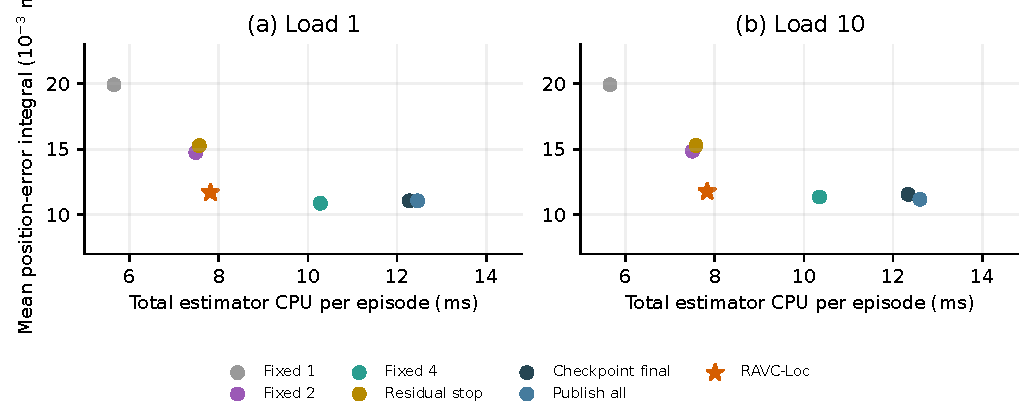
\includegraphics[width=.97\linewidth]{episode_frontier.pdf}
\caption{Retained A20 confirmation work--exposure trade-offs at load factors 1 and 10. Each point averages the same 240 independent episodes; the star marks the policy selected using the separate retained calibration set. Positions are descriptive operating points under the original estimator CPU ledger.}\label{supp:legacy-frontier}
\end{figure}
\begin{figure}[!htbp]\centering
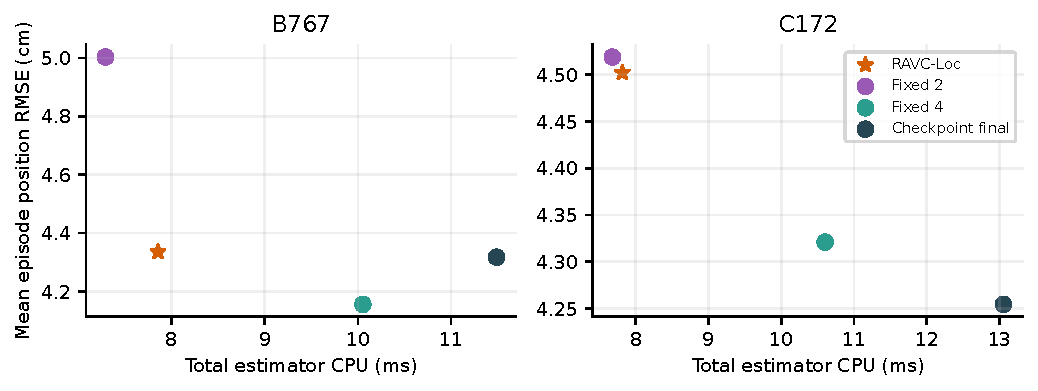
\includegraphics[width=.97\linewidth]{geometry_tradeoff.pdf}
\caption{Retained A20 confirmation trade-offs separated by aircraft geometry at load 10. The common retained calibration mixture determines the selected policy. Aircraft subgroups are descriptive and were not used for reselection.}\label{supp:legacy-geometry}
\end{figure}
\FloatBarrier
\begin{figure}[!htbp]\centering
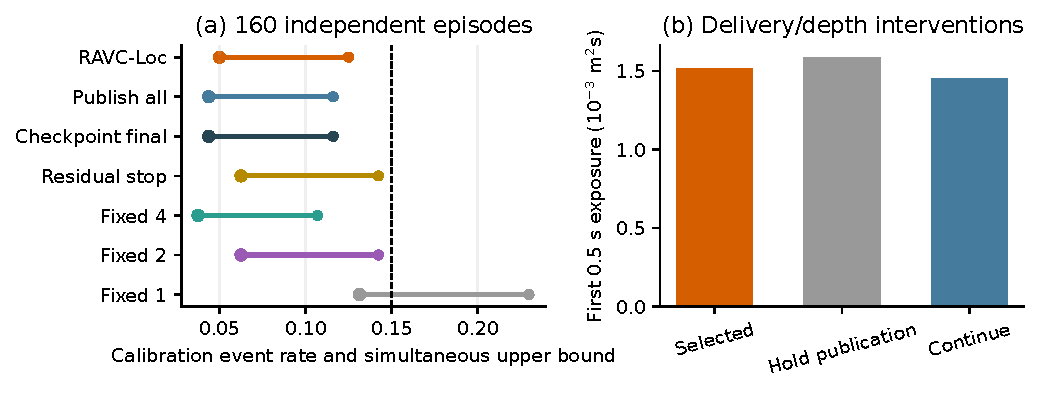
\includegraphics[width=.97\linewidth]{risk_and_delivery.pdf}
\caption{Retained A20 calibration and publication interventions. (a) Point event rates and simultaneous upper bounds for selected controls and RAVC-Loc on 160 independent calibration episodes; the dashed line is $\delta=0.15$. (b) Startup exposure on 240 confirmation episodes at load 10. Holding publication preserves stopping and the final candidate; continuation preserves publication logic and changes iteration depth.}\label{supp:legacy-risk-delivery}
\end{figure}
\begin{figure}[!htbp]\centering
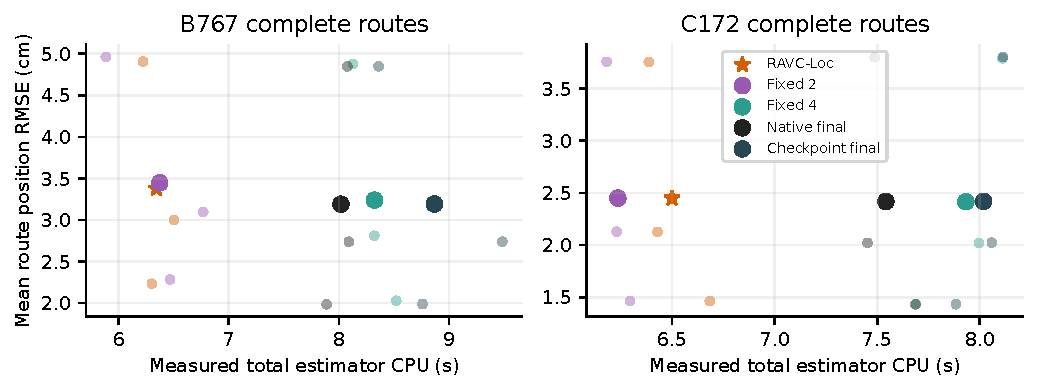
\includegraphics[width=.97\linewidth]{route_tradeoff.pdf}
\caption{Retained A20 complete-route work--error outcomes. Small points are the three retained realizations per aircraft; large points are their method means over 1,980-s routes. Every control uses the same scan cadence and delivery model within this retained block. The original total estimator CPU ledger is preserved.}\label{supp:legacy-route-tradeoff}
\end{figure}
\begin{figure}[!htbp]\centering
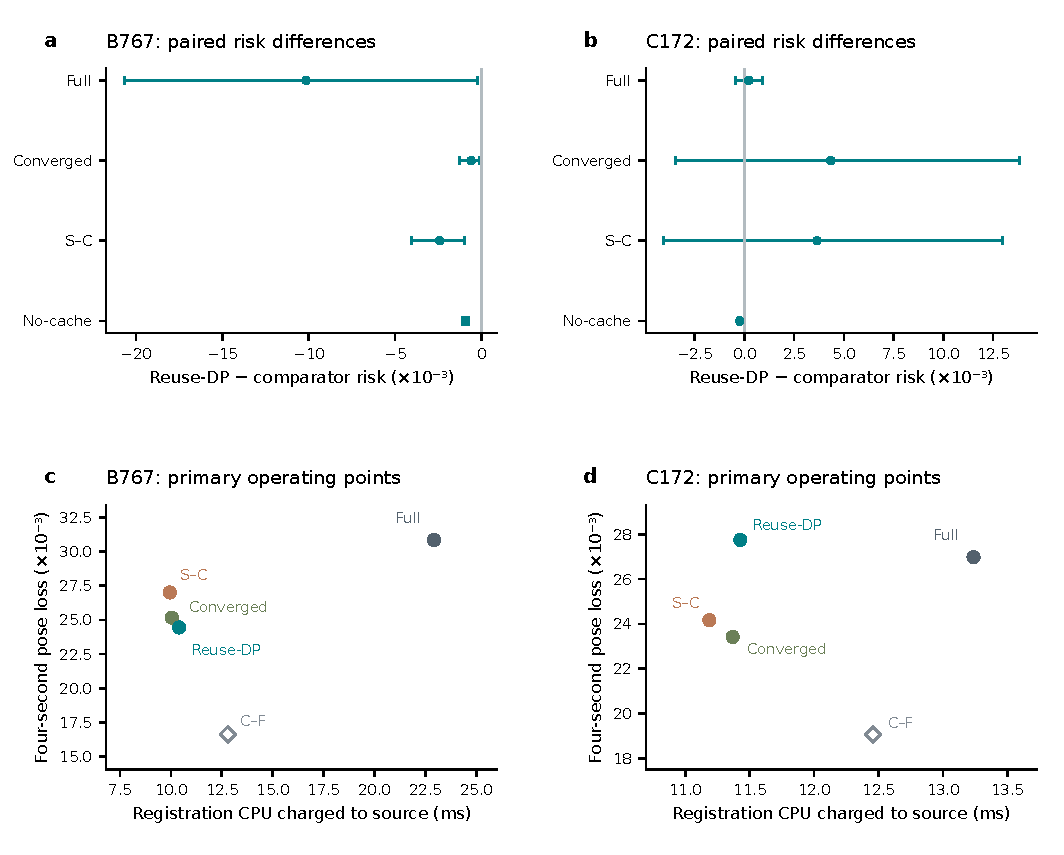
\includegraphics[width=.97\linewidth]{legacy_sources.pdf}
\caption{Retained A19 source-level controls on 240 fresh sources per aircraft at $\lambda=0.3$ and the original primary budget. (a,b) Paired differences in priced risk, Reuse-DP minus the indicated comparator, with pointwise 95\% percentile intervals from 4,000 source-bootstrap resamples. (c,d) Mean geometric loss and measured or replay-charged registration CPU. Filled markers indicate feasibility on all observed primary-budget paths; open diamonds mark the relaxed Converged--Full cascade. These action and reuse controls precede the current checkpoint family.}\label{supp:legacy-sources}
\end{figure}
\begin{figure}[!htbp]\centering
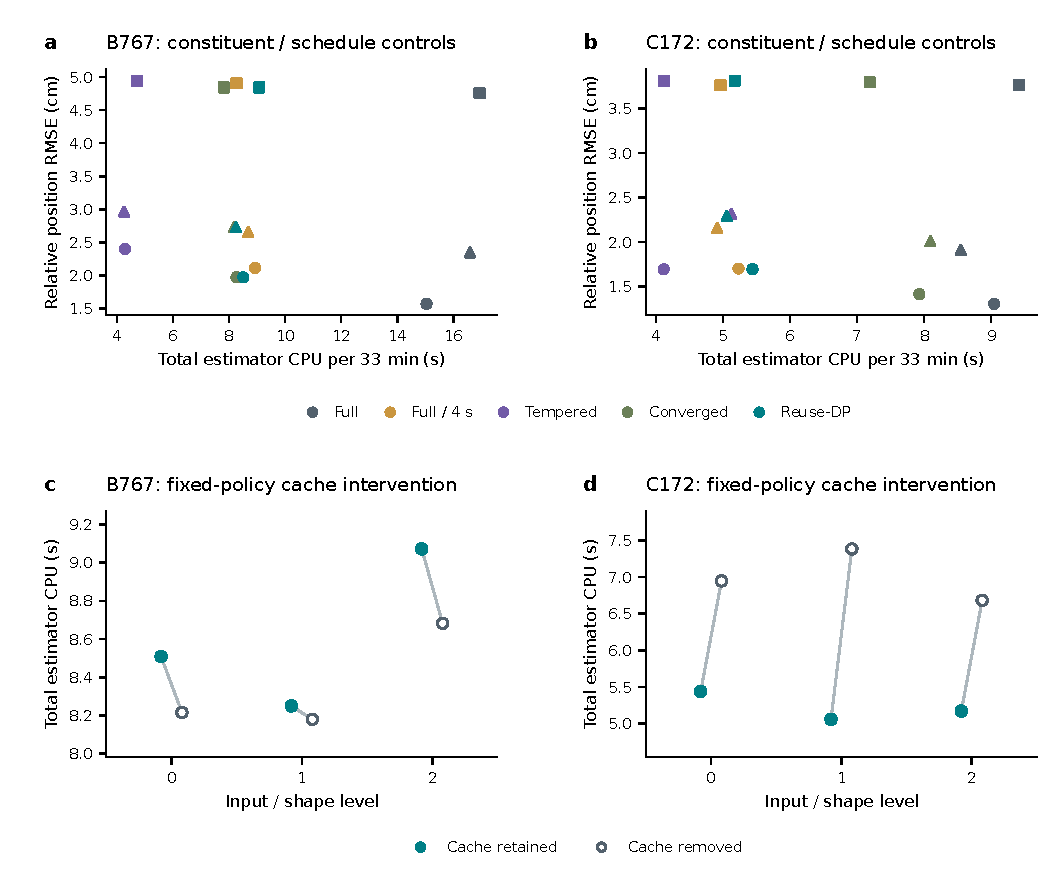
\includegraphics[width=.97\linewidth]{legacy_missions.pdf}
\caption{Retained A19 33-minute route controls and cache interventions. Upper panels compare constituent actions and schedules; lower panels remove reuse at fixed policy across the original input/shape levels. The source archive retains all realizations and the separate route CPU accounting.}\label{supp:legacy-missions}
\end{figure}
\FloatBarrier
\section{Additional physical-platform views}\label{supp:hardware}
Two further original project photographs show platform integration and the aircraft underside. The main R8 paper now includes all four original photographs; these two earlier detail layouts remain for historical continuity. The reproduction bundle preserves the four original JPEGs with their initial dimensions and byte hashes. Photographs provide qualitative engineering context; numerical localization outcomes come from the separately specified simulation inputs.
\begin{figure}[!htbp]\centering
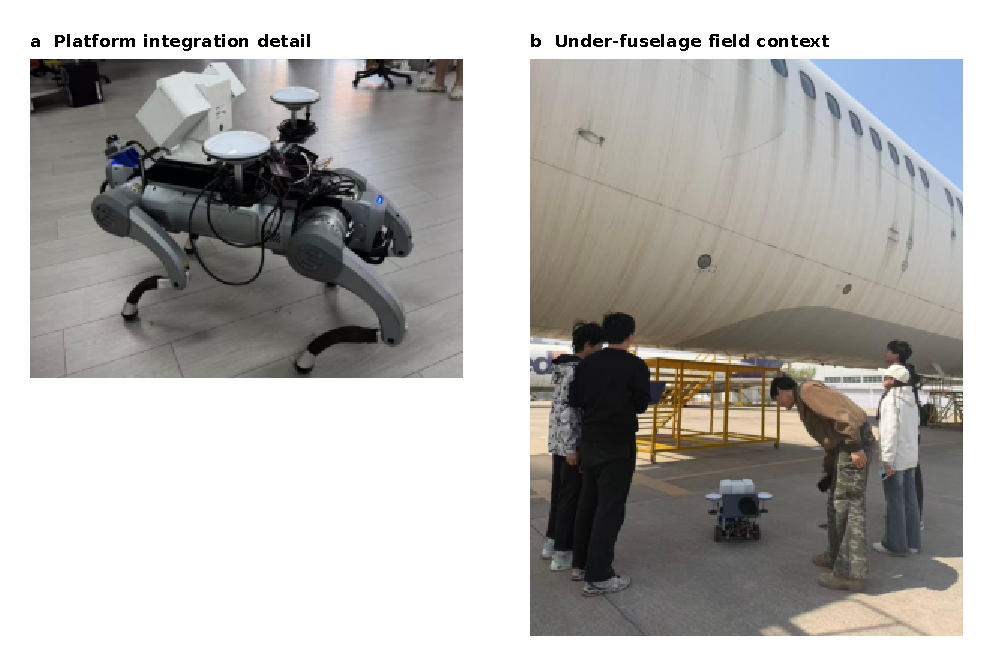
\includegraphics[width=\linewidth]{r7/hardware_details.pdf}
\caption{Additional original physical-platform photographs. (a) Side view of platform integration. (b) Field context beneath the aircraft fuselage. Both images retain their original aspect ratios without cropping, pixel retouching, contrast adjustment or generated content.}\label{supp:hardware-details}
\end{figure}
\FloatBarrier

\end{document}
